\documentclass[11pt]{article}
\setlength\headheight{13.6pt}%
\usepackage[utf8]{inputenc} % Required for inputting international characters
\usepackage[T1]{fontenc} % Output font encoding for international characters
\usepackage{polski}
\usepackage{mathpazo} % Palatino font
\usepackage{graphicx}
\usepackage{fancyhdr}
\usepackage{etoolbox}
\usepackage{blindtext}
\usepackage{geometry}
\usepackage{enumitem}
\geometry{legalpaper, margin=1in}
\usepackage[cleardoublepage=plain]{scrextend}
\graphicspath{ {images/C:\Users\Kuba-PC\Desktop\ProjektIO} }
\pagestyle{fancy}
\fancyhf{}
\rhead{2017/2018}
\lhead{Projekt z Inżynierii Oprogramowania}
\rfoot{Strona \thepage}

\begin{document}
	
	\begin{titlepage} 
	
		\newcommand{\HRule}{\rule{\linewidth}{0.5mm}} % Defines a new command 
		
		\center % Centre everything on the page
		
		%------------------------------------------------
		%	Nagłówki
		%------------------------------------------------
		
		\textsc{\LARGE Akademia Górniczo-Hutnicza im. Stanisława Staszica w Krakowie}\\[1.5cm] % Main heading such as the name of your university/college
		
		\textsc{\Large Projekt z Inżynierii Oprogramowania}\\[0.5cm] % Major heading such as course name
		
		\textsc{\large Informatyka EAIiB 2017/2018}\\[0.5cm] % Minor heading such as course title
		
		%------------------------------------------------
		%	Tytuł
		%------------------------------------------------
		
		\HRule\\[0.4cm]
		
		{\huge\bfseries Lokalizacja w pomieszczeniach bez użycia sygnału GPS}\\[0.4cm] % Title of your document
		
		\HRule\\[1.5cm]
		
		%------------------------------------------------
		%	Authorzy
		%------------------------------------------------
		
		\begin{minipage}{0.4\textwidth}
			\begin{flushleft}
				\large
				\textit{Autorzy}\\
				Jakub \textsc{Kacorzyk} \\
				Bartłomiej \textsc{Łazarczyk}
			\end{flushleft}
		\end{minipage}
		~
		\begin{minipage}{0.4\textwidth}
			\begin{flushright}
				\large
				\textit{Prowadzący}\\
				dr inż. Radosław \textsc{Klimek} % Supervisor's name
			\end{flushright}
		\end{minipage}
		
		%------------------------------------------------
		%	Logo
		%------------------------------------------------
		
		\vfill\vfill
		
\includegraphics[scale=1.0]{logo.jpg}
		
		%------------------------------------------------
		%	Data
		%------------------------------------------------
		
		\vfill\vfill\vfill % Position the date 3/4 down the remaining page
		
		{\large\today} 
		
		%----------------------------------------------------------------------------------------
		
		\vfill % Push the date up 1/4 of the remaining page
		
	\end{titlepage}
	
	\tableofcontents
	\cleardoublepage
	\setcounter{page}{2}
	
	
	\section{Streszczenie}
	Projekt modeluje działanie aplikacji mobilnej lokalizującej użytkownika w środowisku indoor. 
	Głównym założeniem systemu jest wyznaczenie oraz śledzenie lokalizacji klienta bez udziału sygnału GPS. Aby to osiągnąć wykorzystywane są urządzenia dostępu do sieci Wi-Fi znajdujące się w budynku, maszty telefonii komórkowej oraz urządzenia pomiarowe dostępne w telefonie takie jak akcelerometr, magnetometr, barometr.
	
	Wyznaczanie pozycji startowej zależy od dostępu do internetu oraz otaczających sieci Wi-Fi.
	W przypadku niespełnienia powyższych warunków wyznaczany jest potencjalny obszar na podstawie informacji uzyskanych z sieci komórkowej. Im więcej nadajników sieci komórkowej użytkownika w pobliżu, tym dokładniejszy jest wyznaczony obszar.
	Po ustaleniu pozycji bazowej, aplikacja opiera się na urządzeniach pomiarowych dostępnych  w telefonie do śledzenia zmiany jego położenia. W przypadku otrzymania kolejnej informacji od urządzenia zewnętrznego, porównywana jest ona ze zmianami zarejestrowanymi przez telefon oraz wyznaczany jest dopuszczalny błąd pomiarowy dla urządzenia które tą informację przesłało. Ostateczną lokalizację wyznacza specjalny algorytm na podstawie wszystkich uzyskanych w danym momencie danych.
	
	\section{Lista obiektów}
	\begin{itemize}
		\item Wi-Fi
		\item Aplikacja mobilna
		\item Użytkownik
		\item Barometr
		\item Akcelerometr
		\item Magnetometr
		\item Maszty telefonii komórkowej
	\end{itemize}
	
	\section{Lista bodźców}
	\begin{itemize}
		\item Sygnały taktowane zegarem
		\begin{enumerate}
			
		\item Żądanie udostępnienia informacji o urządzeniu punktu dostępu wi-fi oraz o otrzymywanym sygnale
	    \item Żądanie określenia lokalizacji wysyłane przez aplikację mobilną
		\item Żądanie wyznaczenia kierunku przez magnetometr
		\item Żądanie wyznaczenia ciśnienia przez barometr
		\item Żądanie wyznaczenia zmiany prędkości przez akcelerometr
		
		\end{enumerate}
		\item Sygnały sterujące
		\begin{enumerate}
		\item Zlecenie lokalizacji urządzenia przez użytkownika
		\item Zlecenie wyznaczenia przebytej trasy przez użytkownika
		\item Zlecenie śledzenia lokalizacji przez użytkownika
	    \item Zwrócenie wyznaczonej trasy przez system obsługi lokalizacji
		\item Zwrócenie danych o położeniu  przez system obsługi lokalizacji
				
		\end{enumerate}
		\item Sygnały przepływu danych
		\begin{enumerate}
		\item	Dane o zmianach ciśnienia pobierane z barometra.
		\item	Dane o zmianach kierunku pobierane z magnetometra.
		\item	Dane położenia względem masztów telefonii komórkowej.
		\item	Dane o zmianach prędkości poruszania się pobierane z akcelerometra.
		\item	Dane o urządzeniu pobierane z urządzenia Wi-Fi
		\item	Dane o sygnale pobierane z urządania Wi-Fi
				
		\end{enumerate}
	\end{itemize}
	\newpage
	\section{Diagram kontekstowy}
    \begin{center}
	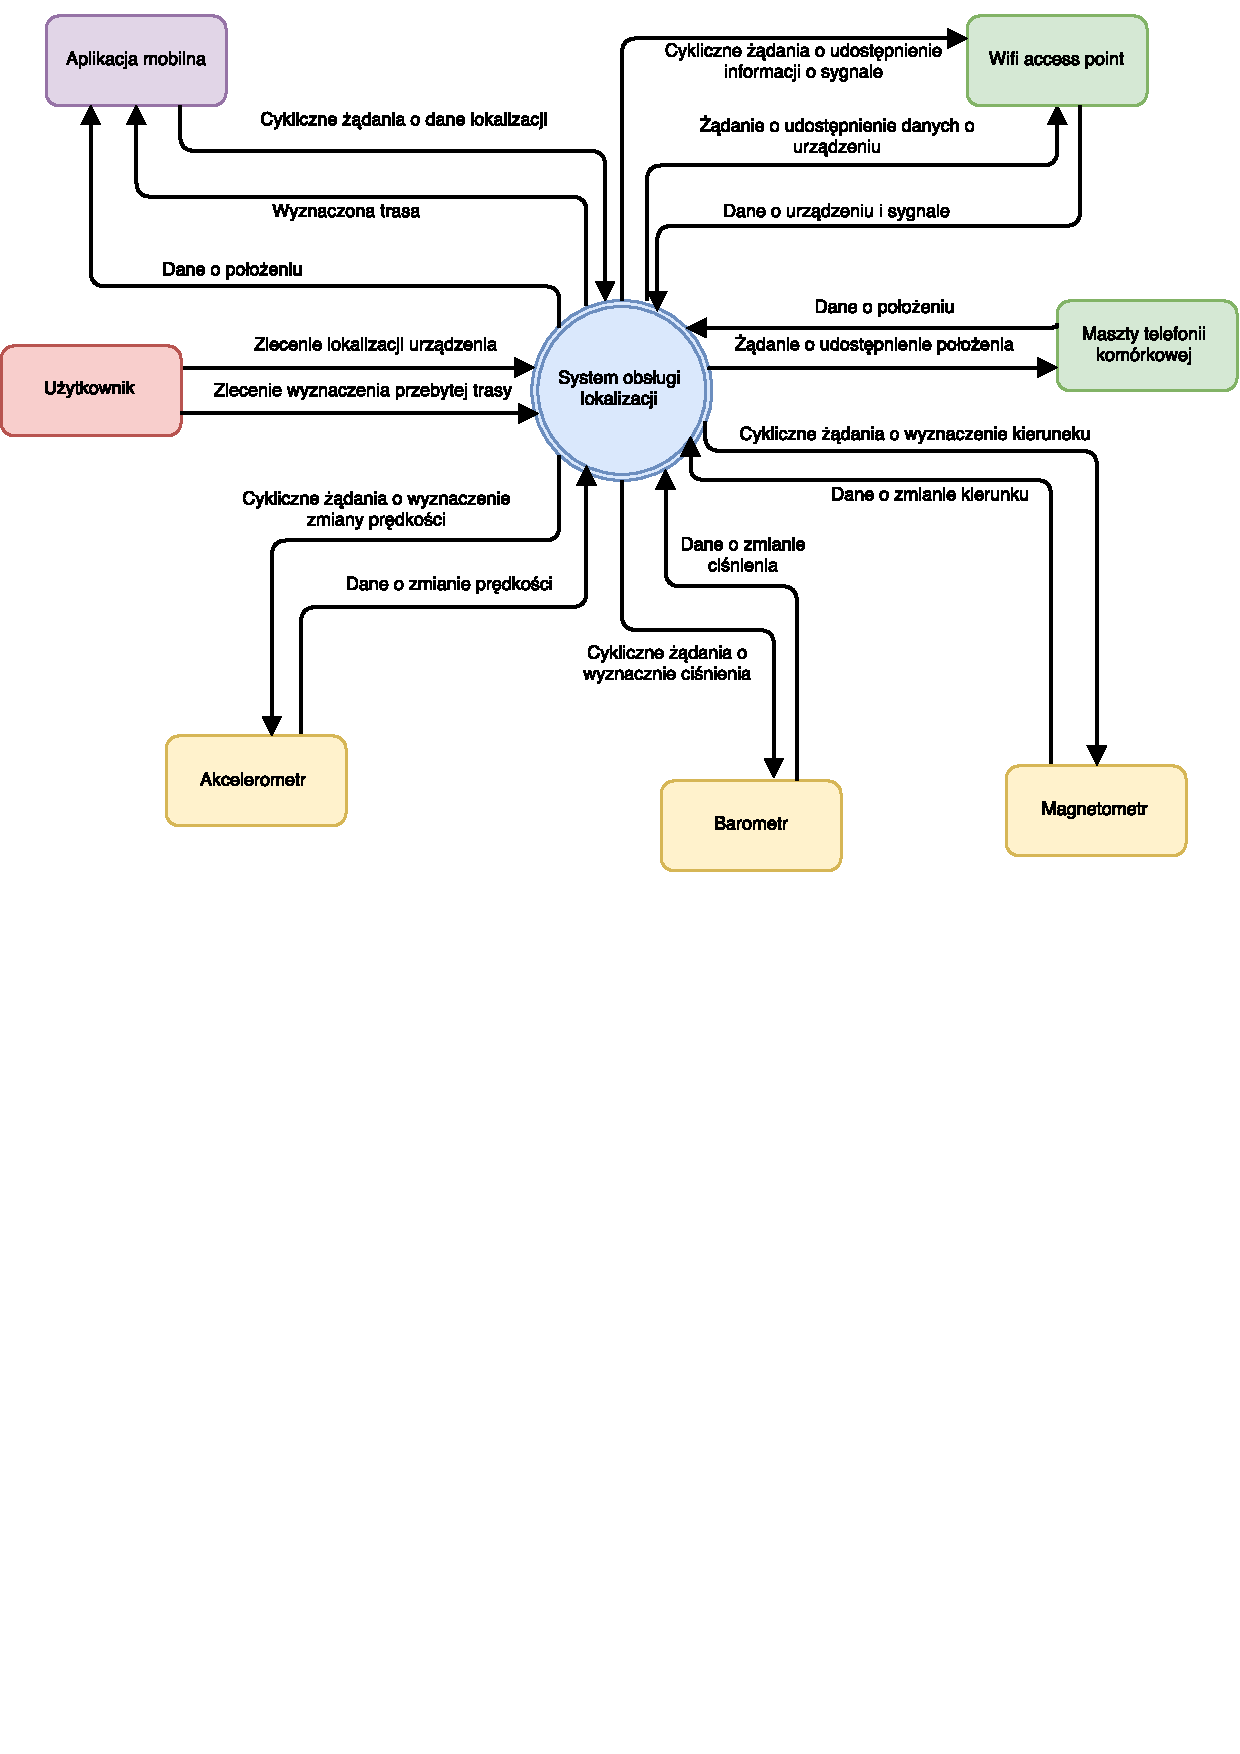
\includegraphics[scale=0.9]{DiagramKontekstowy.pdf}
	\end{center}
	\newpage
	\section{DFD poziom 0}
	\begin{center}
		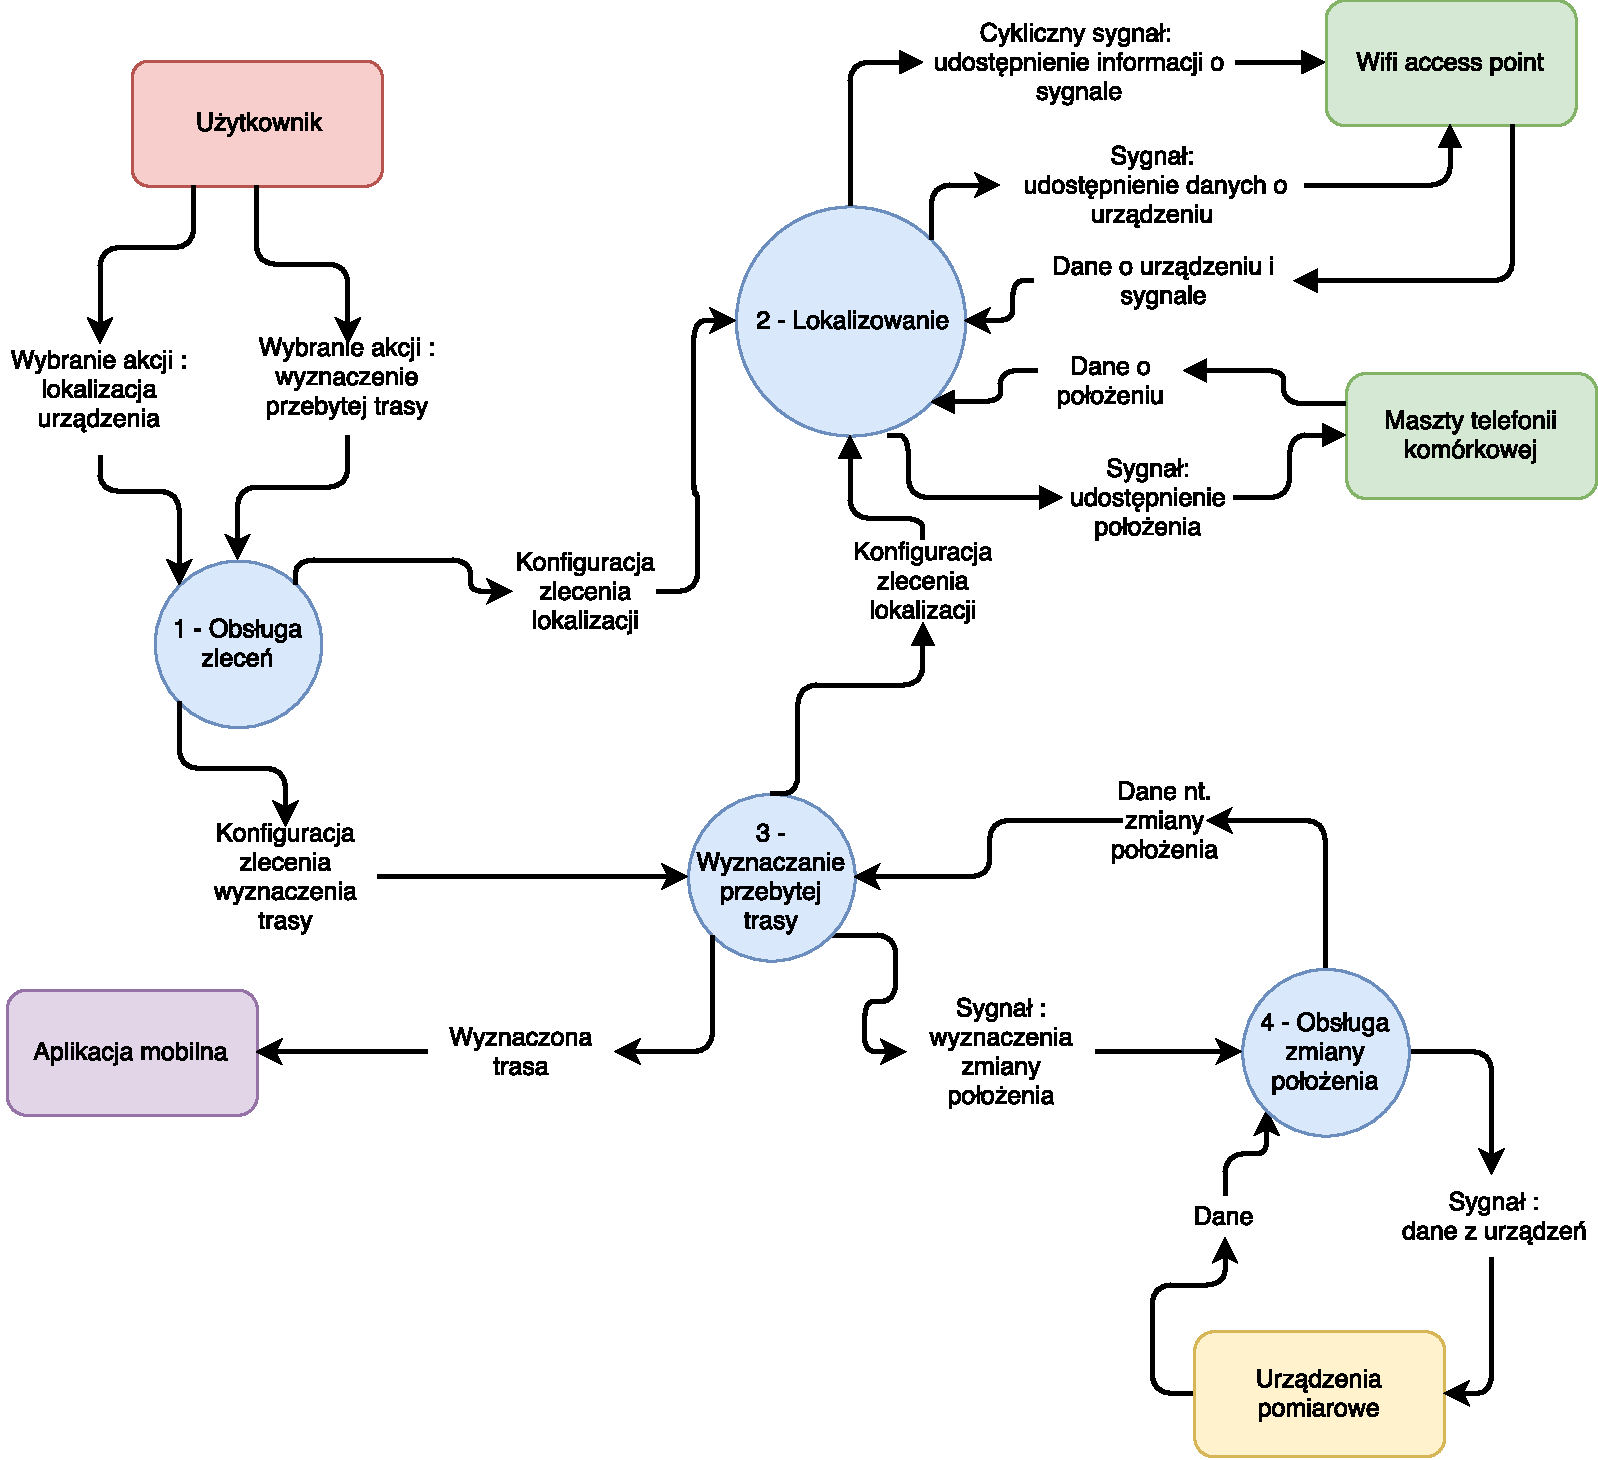
\includegraphics[scale=0.8]{DFD0.pdf}
	\end{center}
	\newpage
	\section{DFD poziom 1 dekompozycje}
	\subsection{DFD 1 Osługa zleceń}
	\begin{center}
		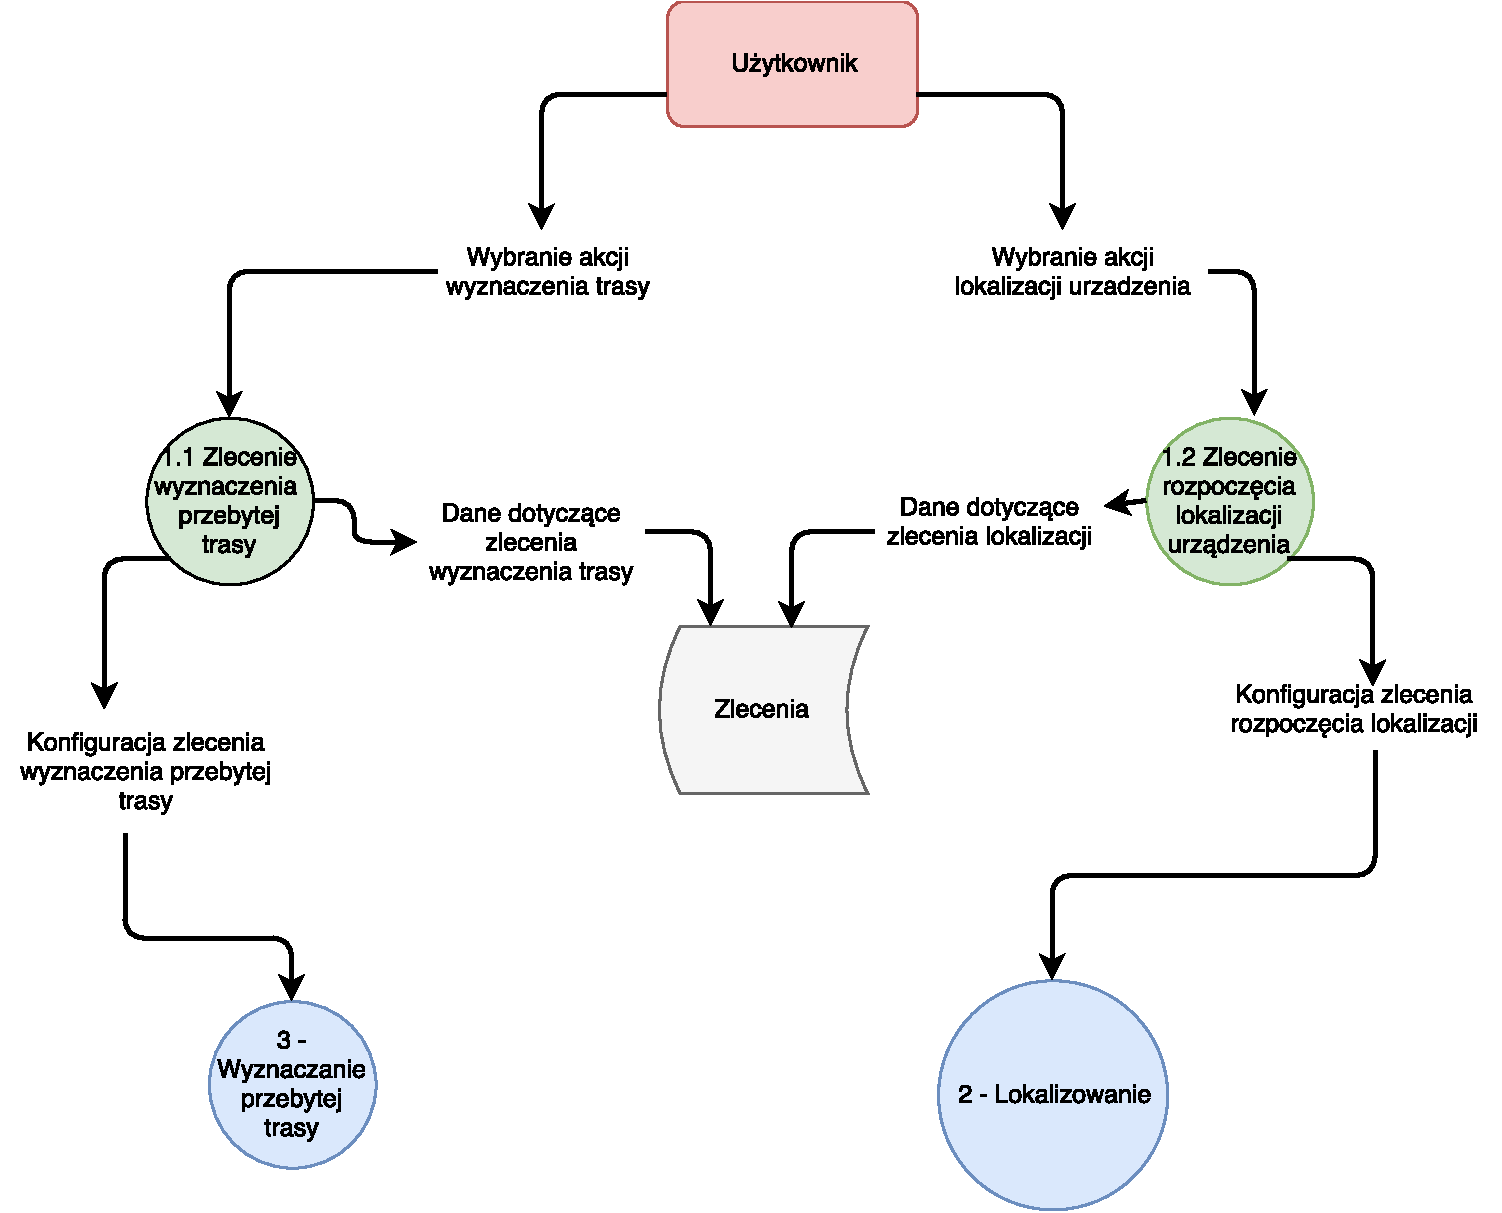
\includegraphics[scale=0.7]{DFD1.pdf}
	\end{center}
	\subsection{DFD 2 Lokalizowanie}
	\begin{center}
		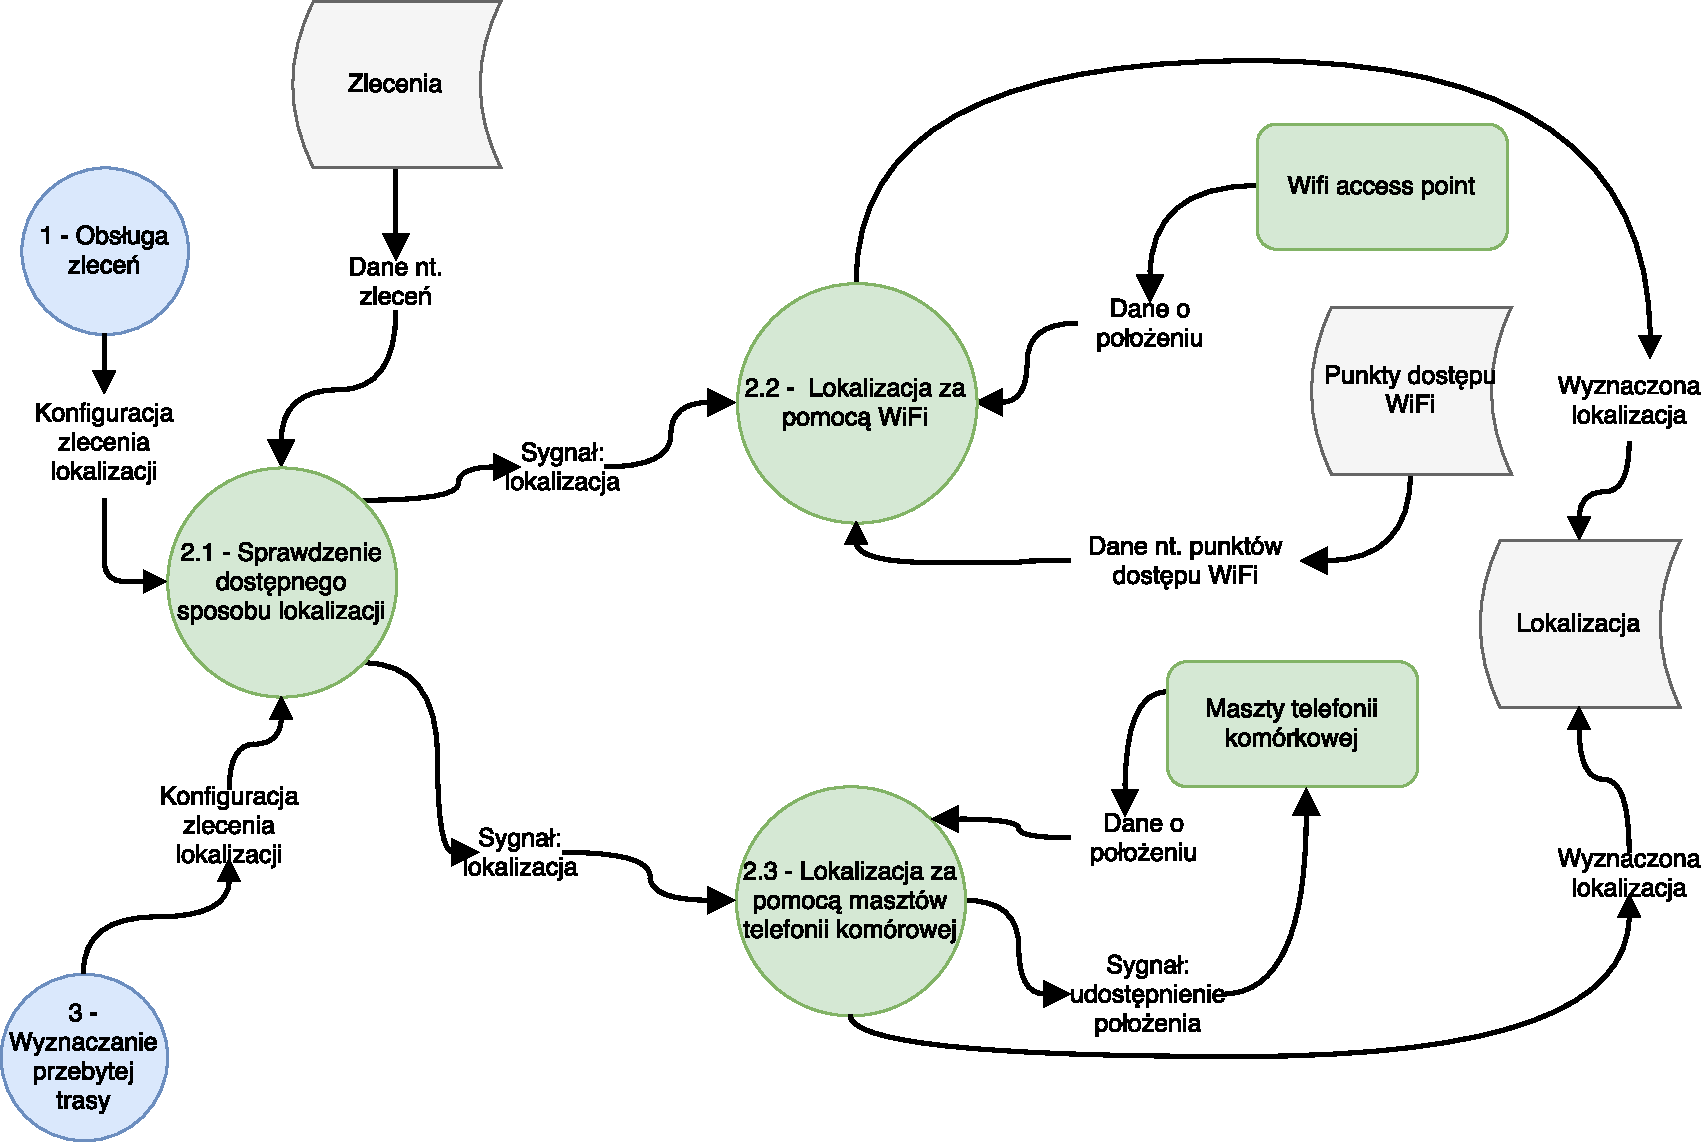
\includegraphics[scale=0.6]{DFD2.pdf}
	\end{center}
	\newpage
	\subsection{DFD 3 Wyznaczanie przebytej trasy}
	\begin{center}
		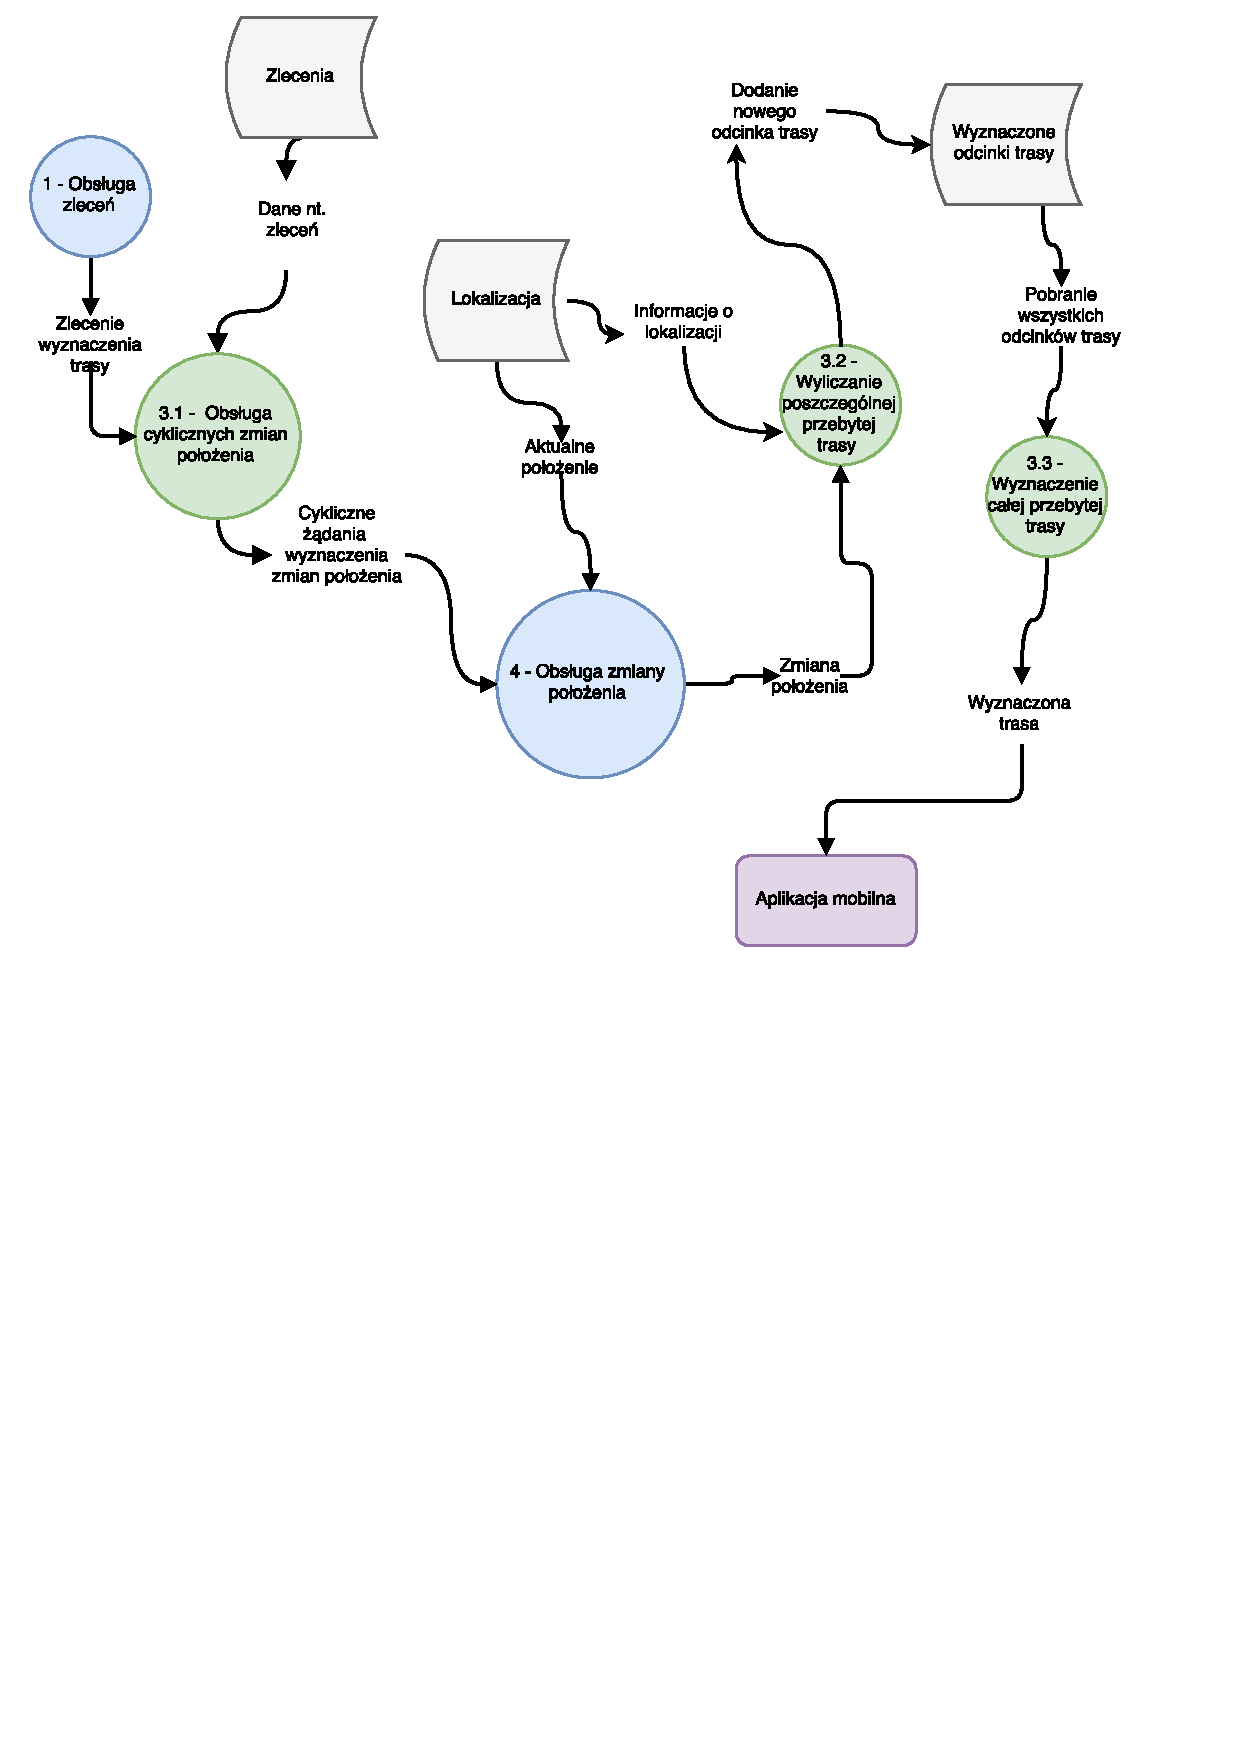
\includegraphics[scale=0.6]{DFD3.pdf}
	\end{center}
	\subsection{DFD 4 Obsługa zmiany położenia}
	\begin{center}
		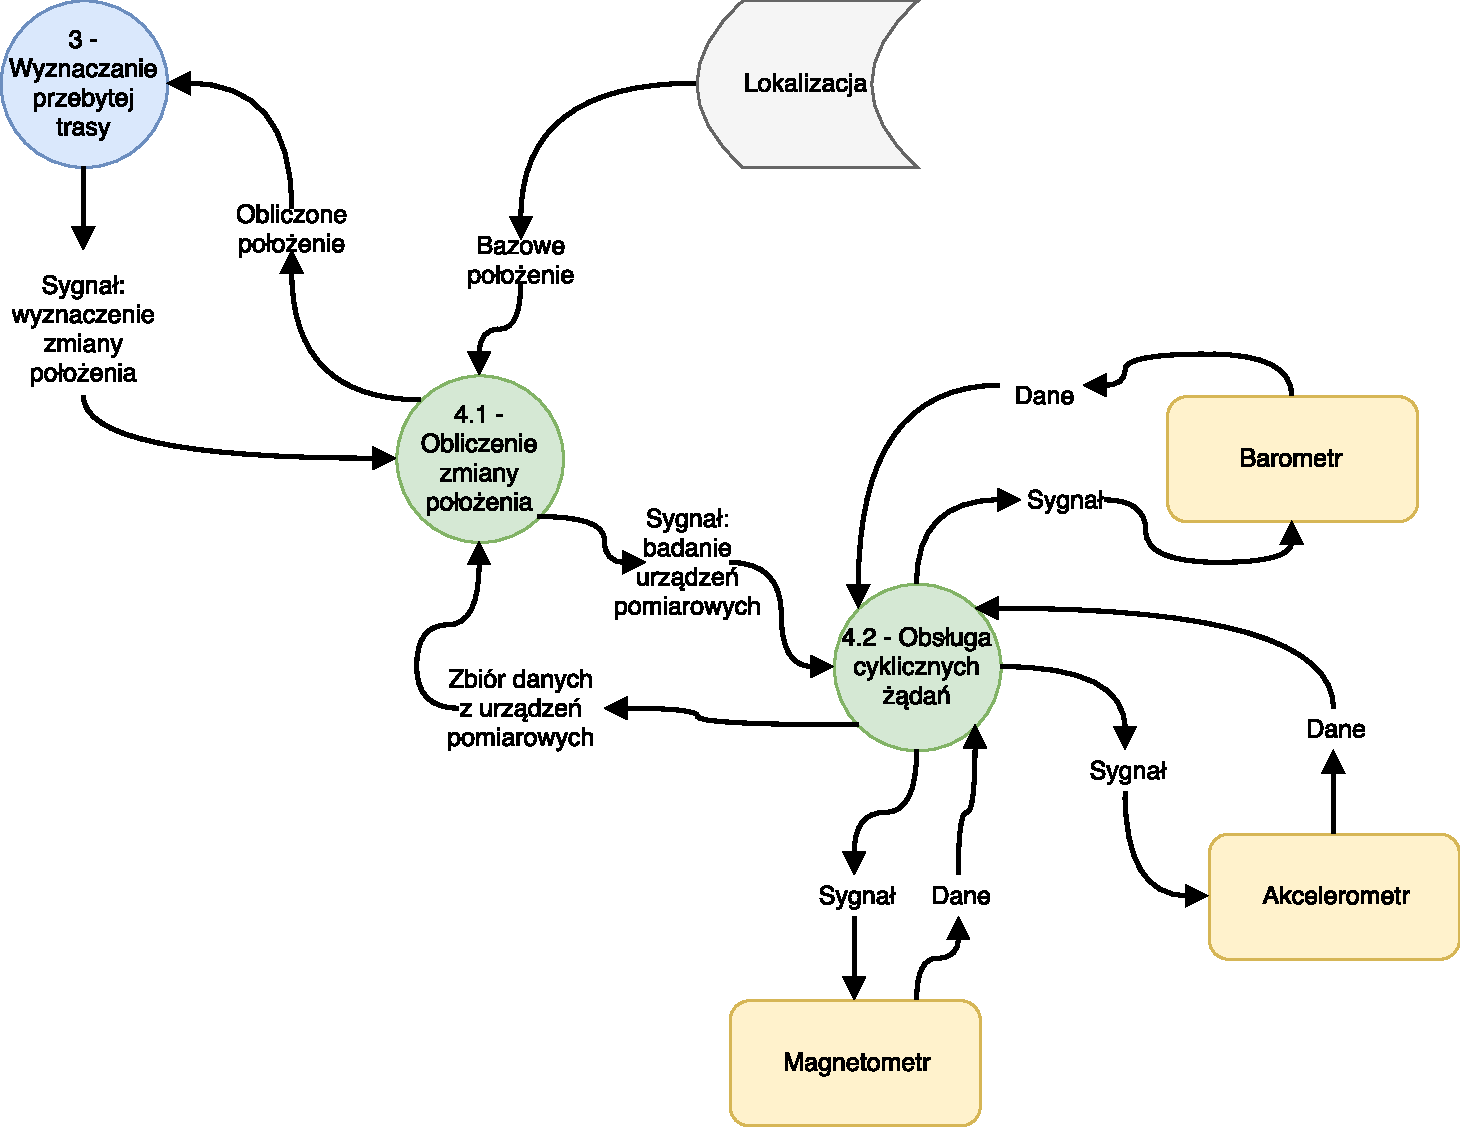
\includegraphics[scale=0.7]{DFD4.pdf}
	\end{center}
	\newpage
	\section{DFD poziom 2 dekompozycje}
	\subsection{DFD 1.1 Zlecenie wyznaczenia przebytej trasy }
	\begin{center}
		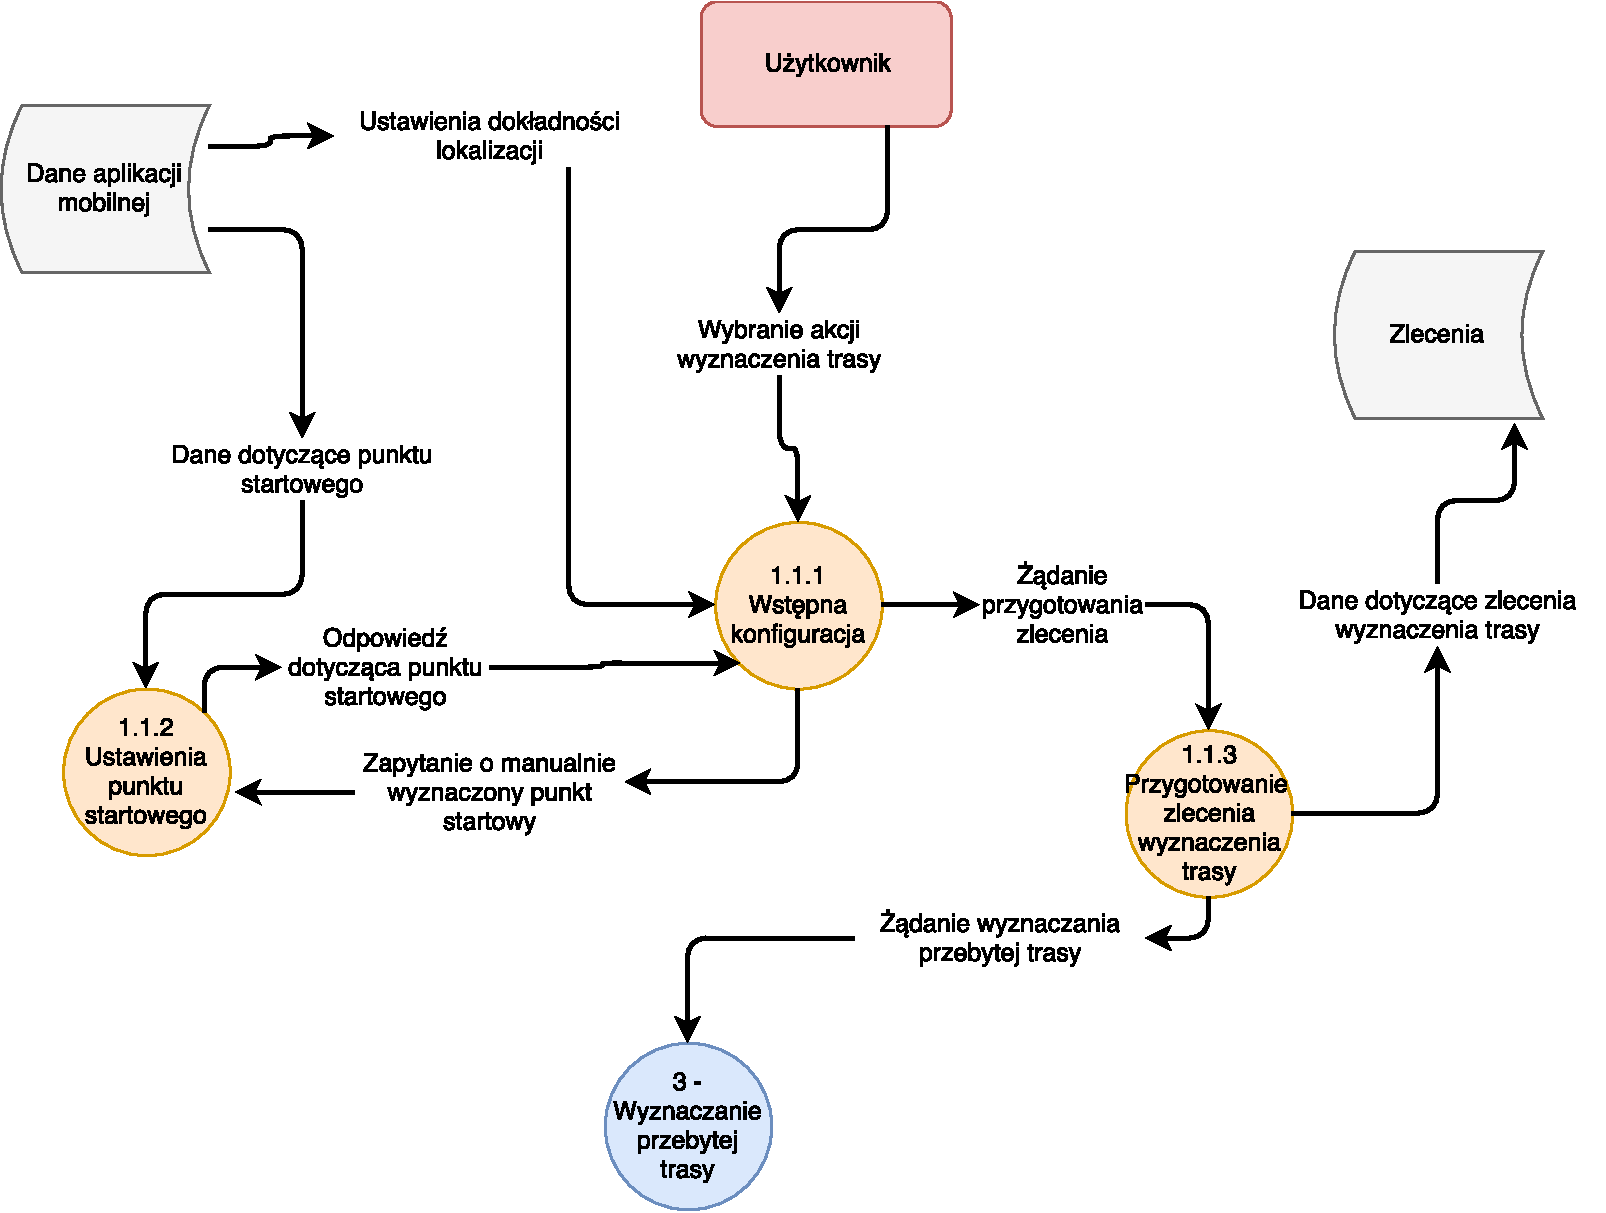
\includegraphics[scale=0.6]{DFD11.pdf}
	\end{center}
	\subsection{DFD 1.2 Zlecenie rozpoczęcia lokalizacji urządzenia}
	\begin{center}
		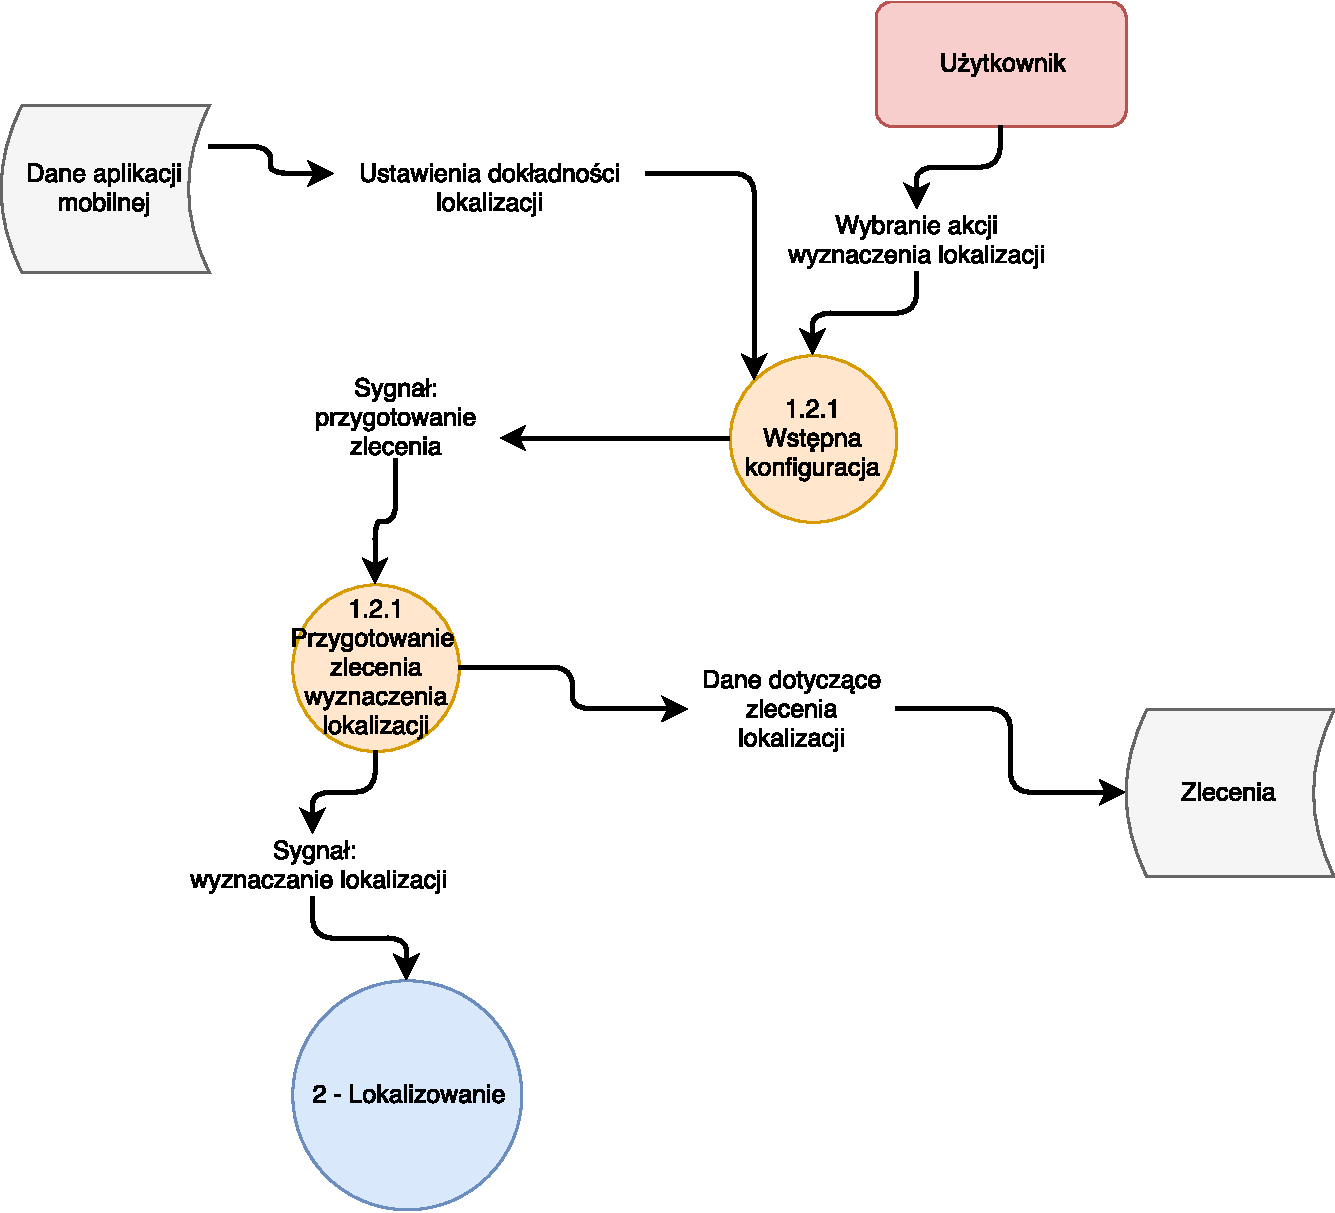
\includegraphics[scale=0.7]{DFD12.pdf}
	\end{center}
	\newpage
	\subsection{DFD 2.1 Sprawdzenie dostępnego sposobu lokalizaci}
	\begin{center}
		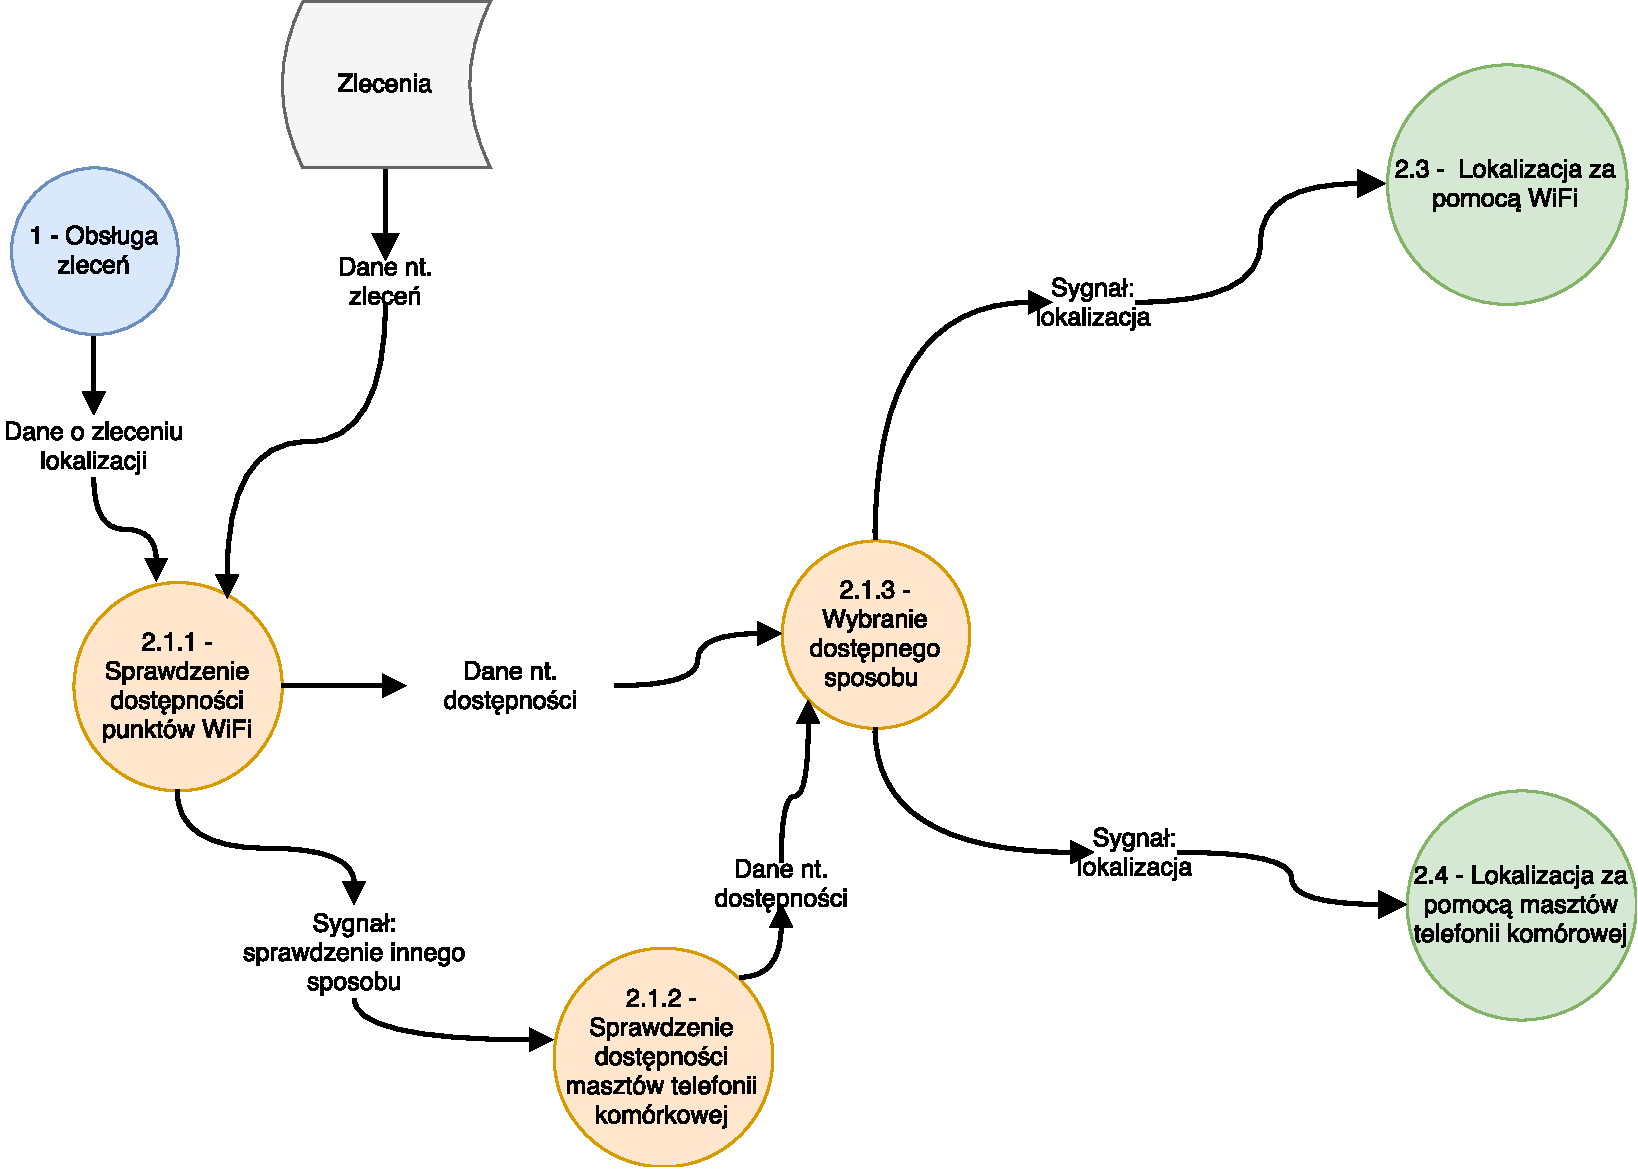
\includegraphics[scale=0.6]{DFD21.pdf}
	\end{center}
	\subsection{DFD 2.2 Lokalizacja za pomocą WiFi}
	\begin{center}
		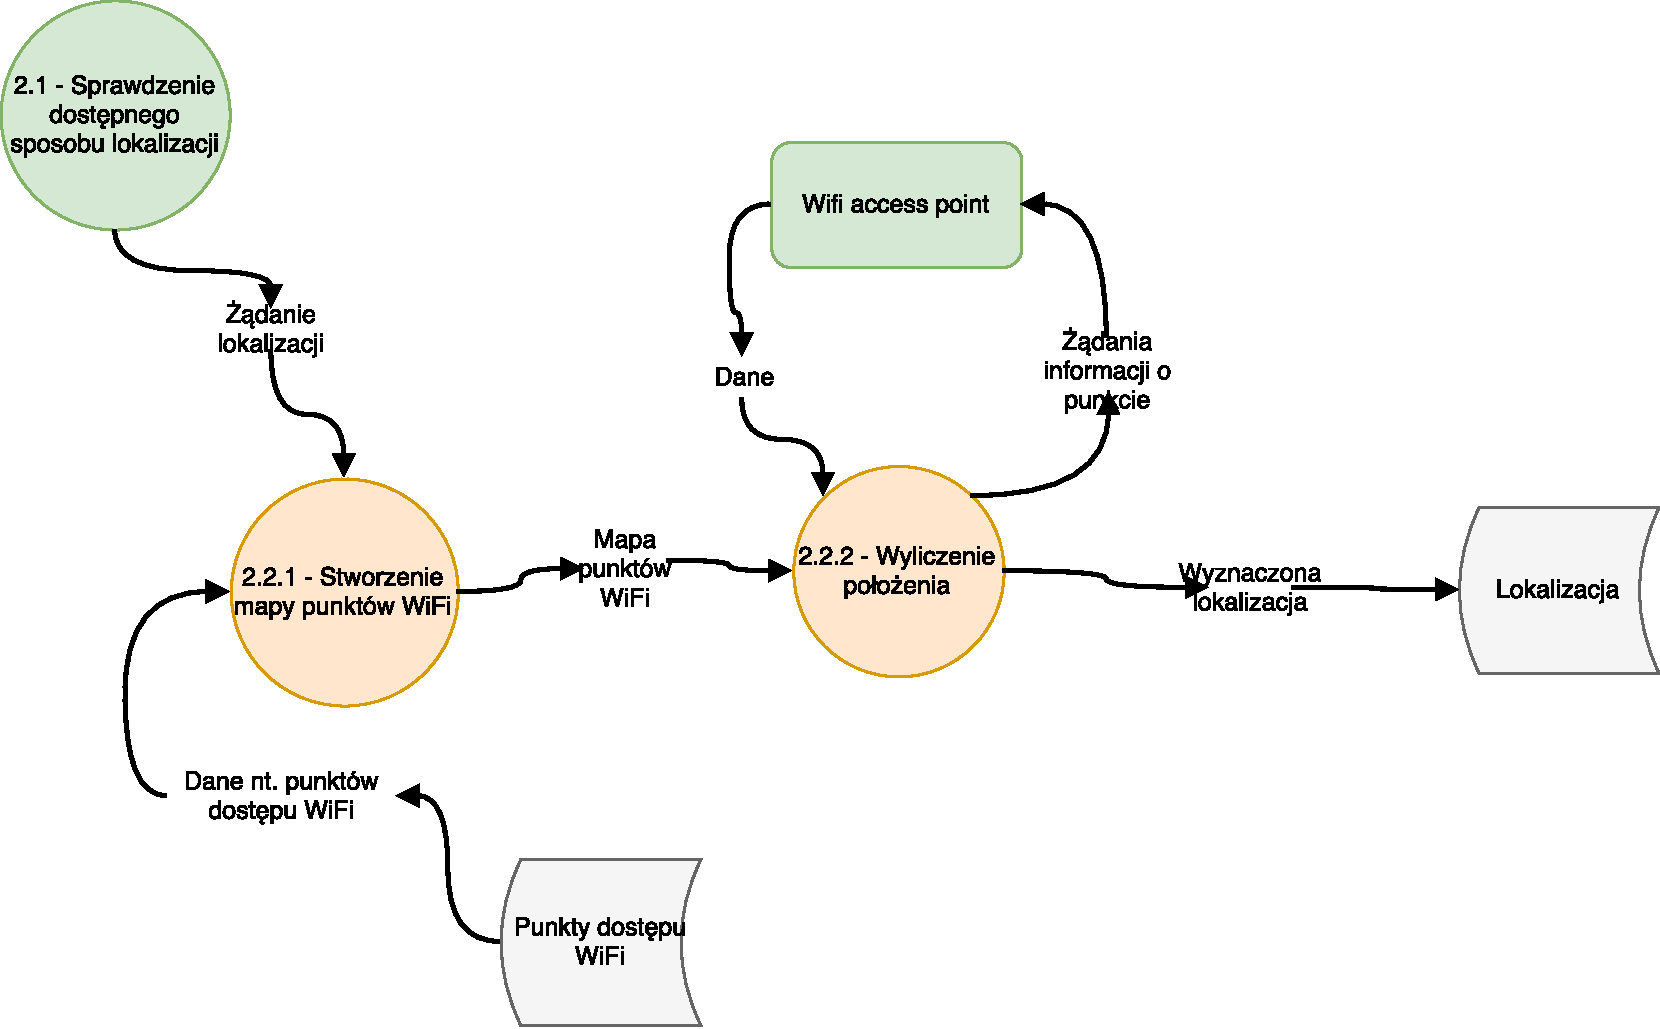
\includegraphics[scale=0.6]{DFD22.pdf}
	\end{center}
	\newpage
	\subsection{DFD 2.3 Lokalizacja za pomocą masztów telefonii komórkowej}
	\begin{center}
		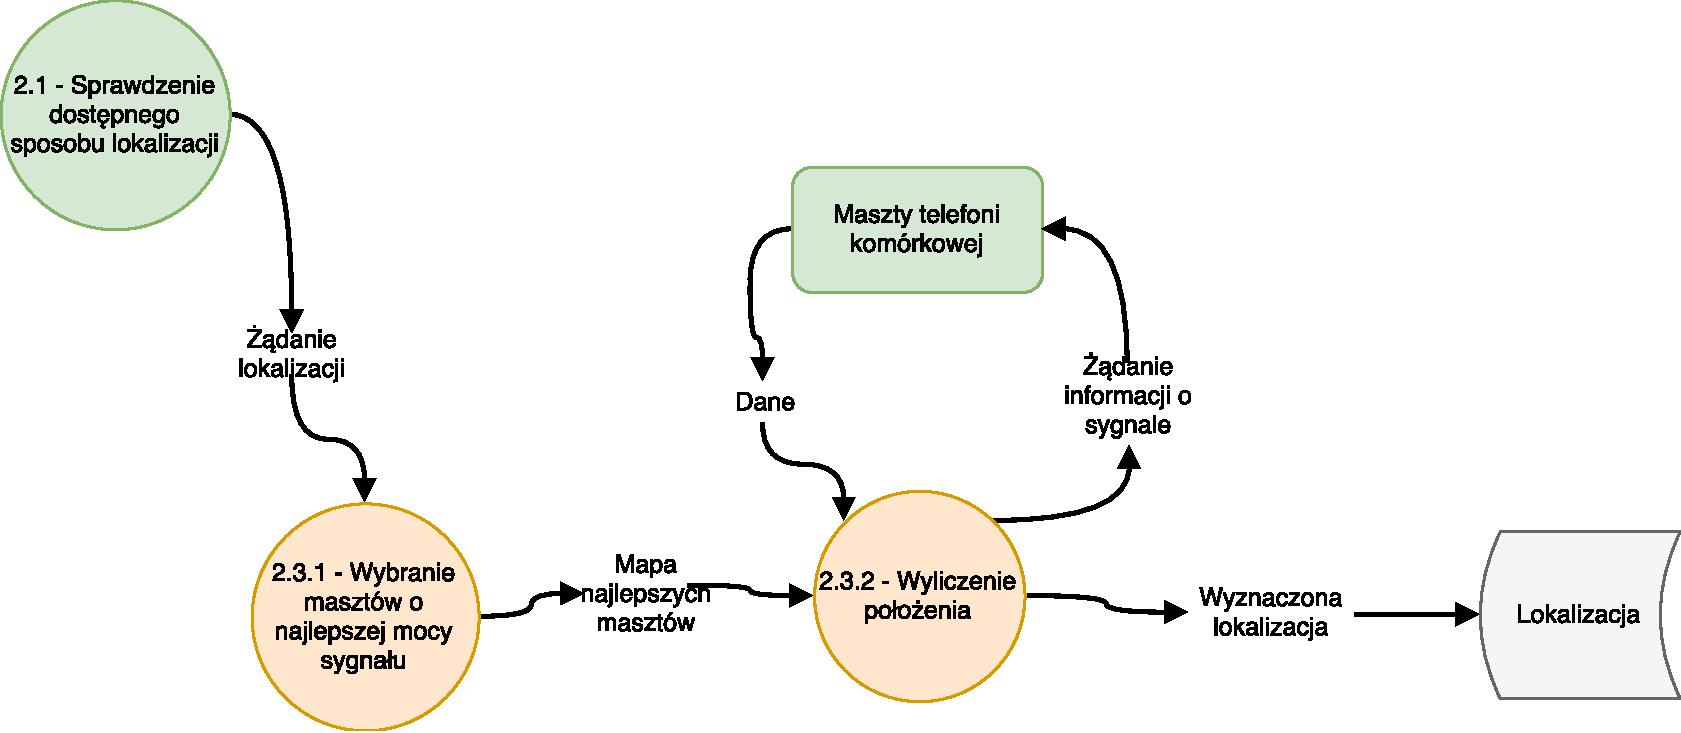
\includegraphics[scale=0.65]{DFD23.pdf}
	\end{center}
	\subsection{DFD 3.1 Obsługa cyklicznych zmian położenia}
	\begin{center}
		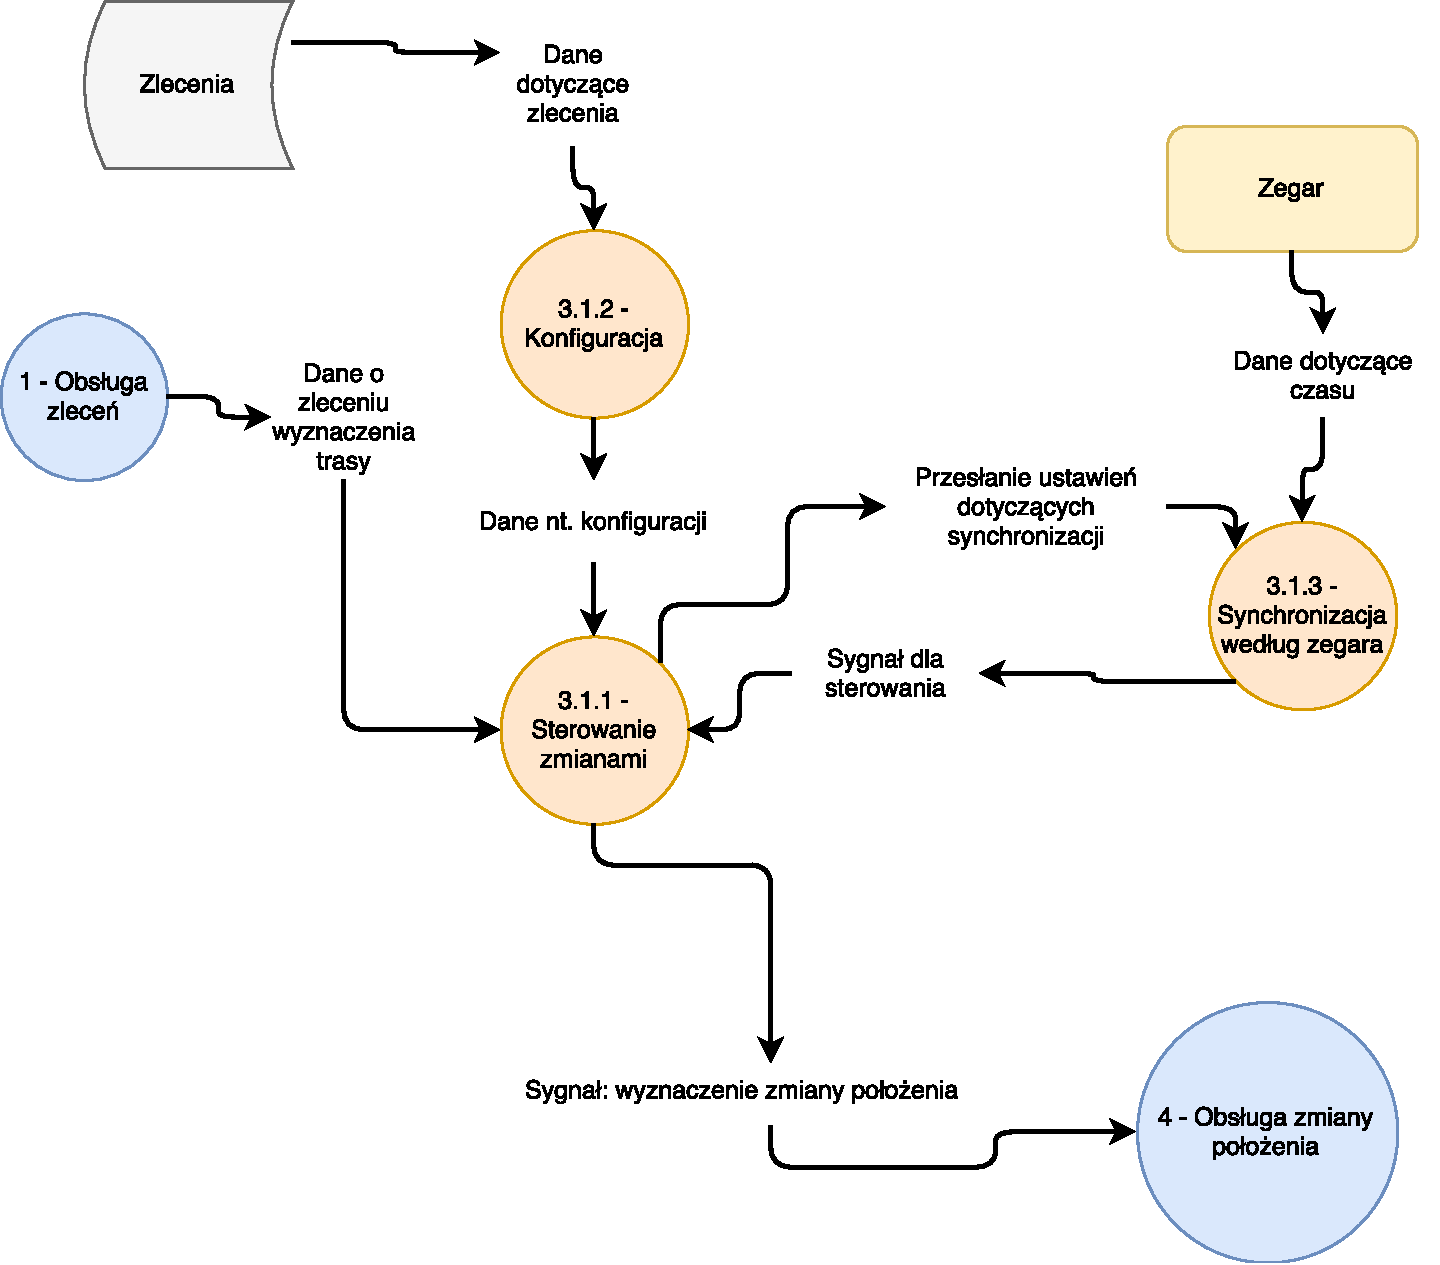
\includegraphics[scale=0.65]{DFD31.pdf}
	\end{center}
	\newpage
	\subsection{DFD 3.2 Wyliczanie odcinka przebytej trasy}
	\begin{center}
		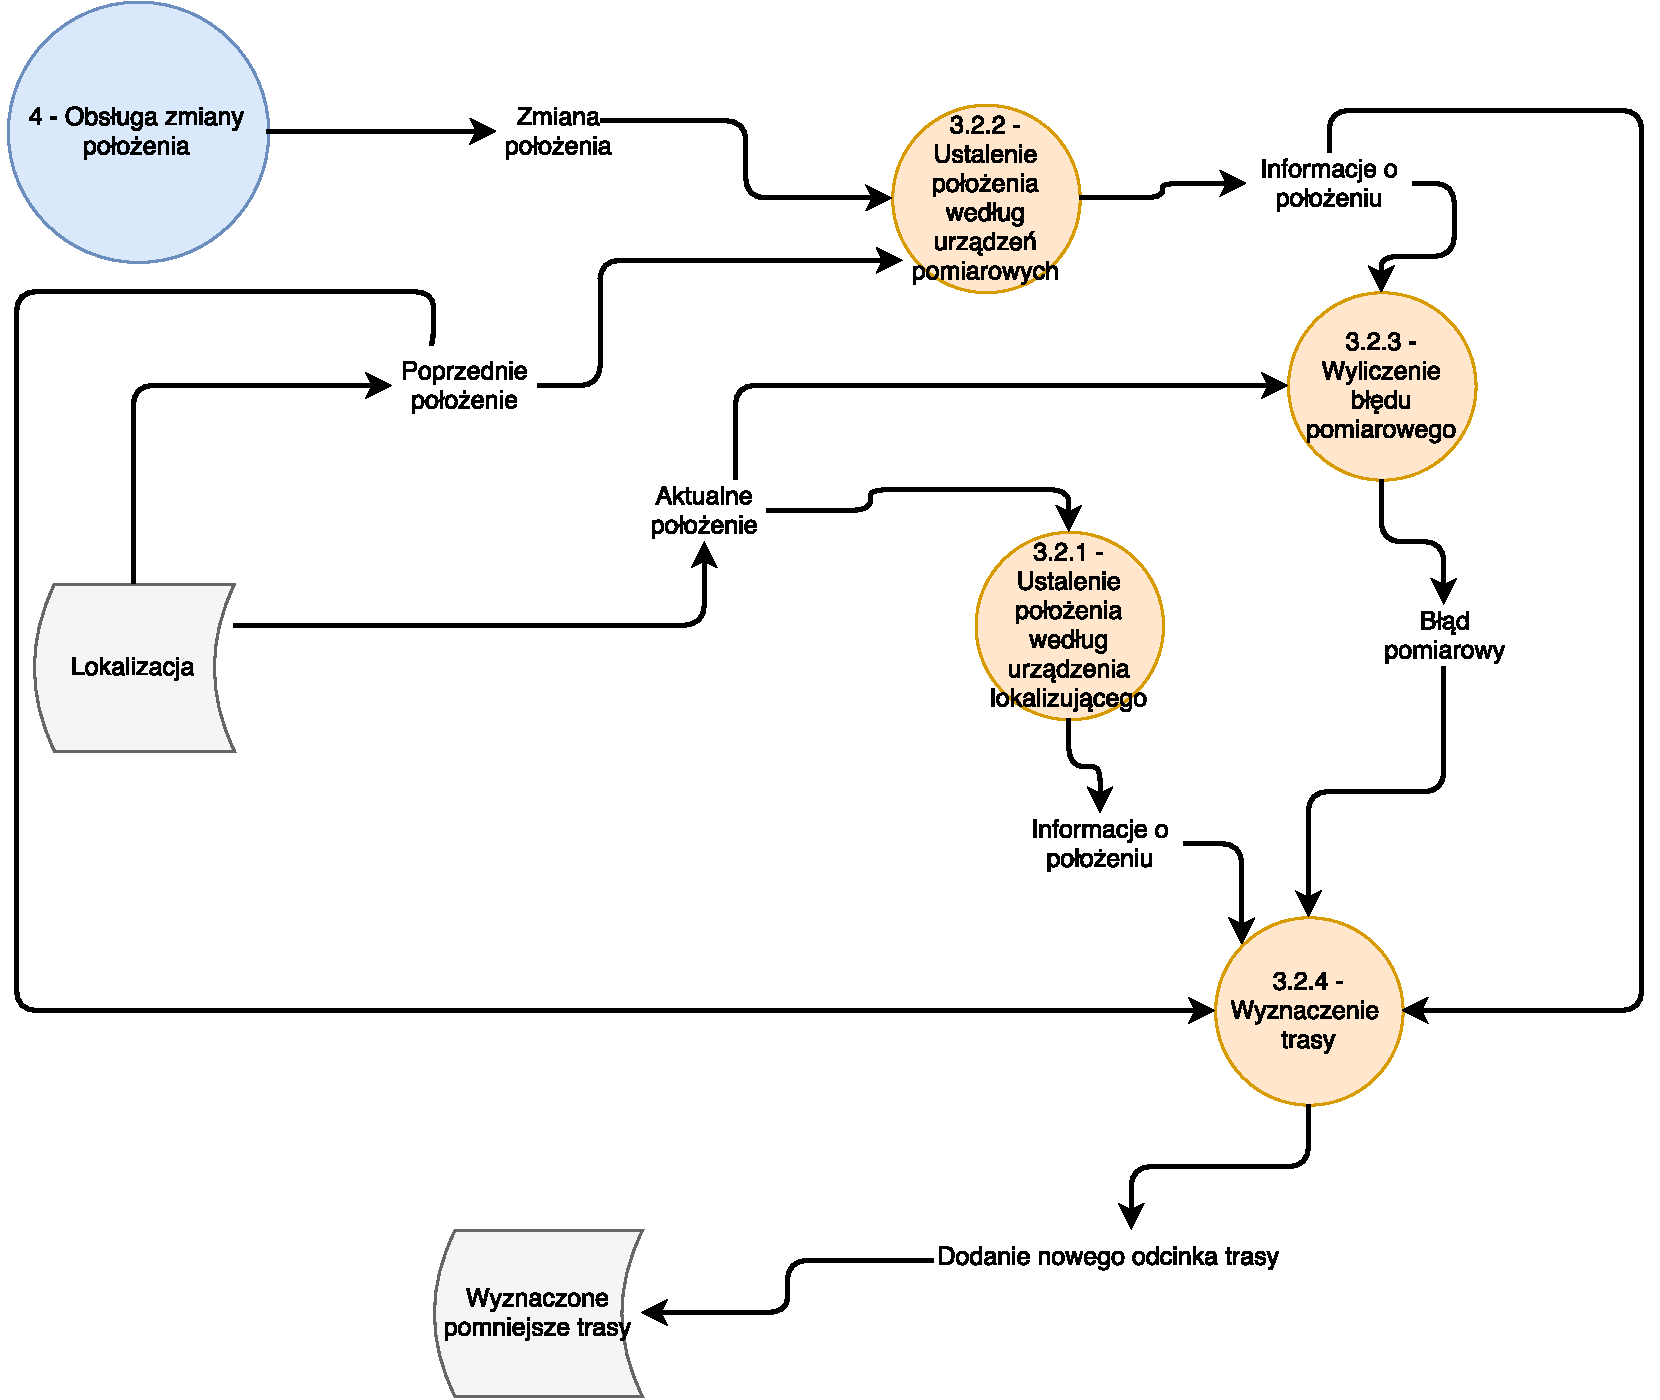
\includegraphics[scale=0.65]{DFD32.pdf}
	\end{center}
	\subsection{DFD 3.3 Wyznaczanie całej przebytej trasy}
	\begin{center}
		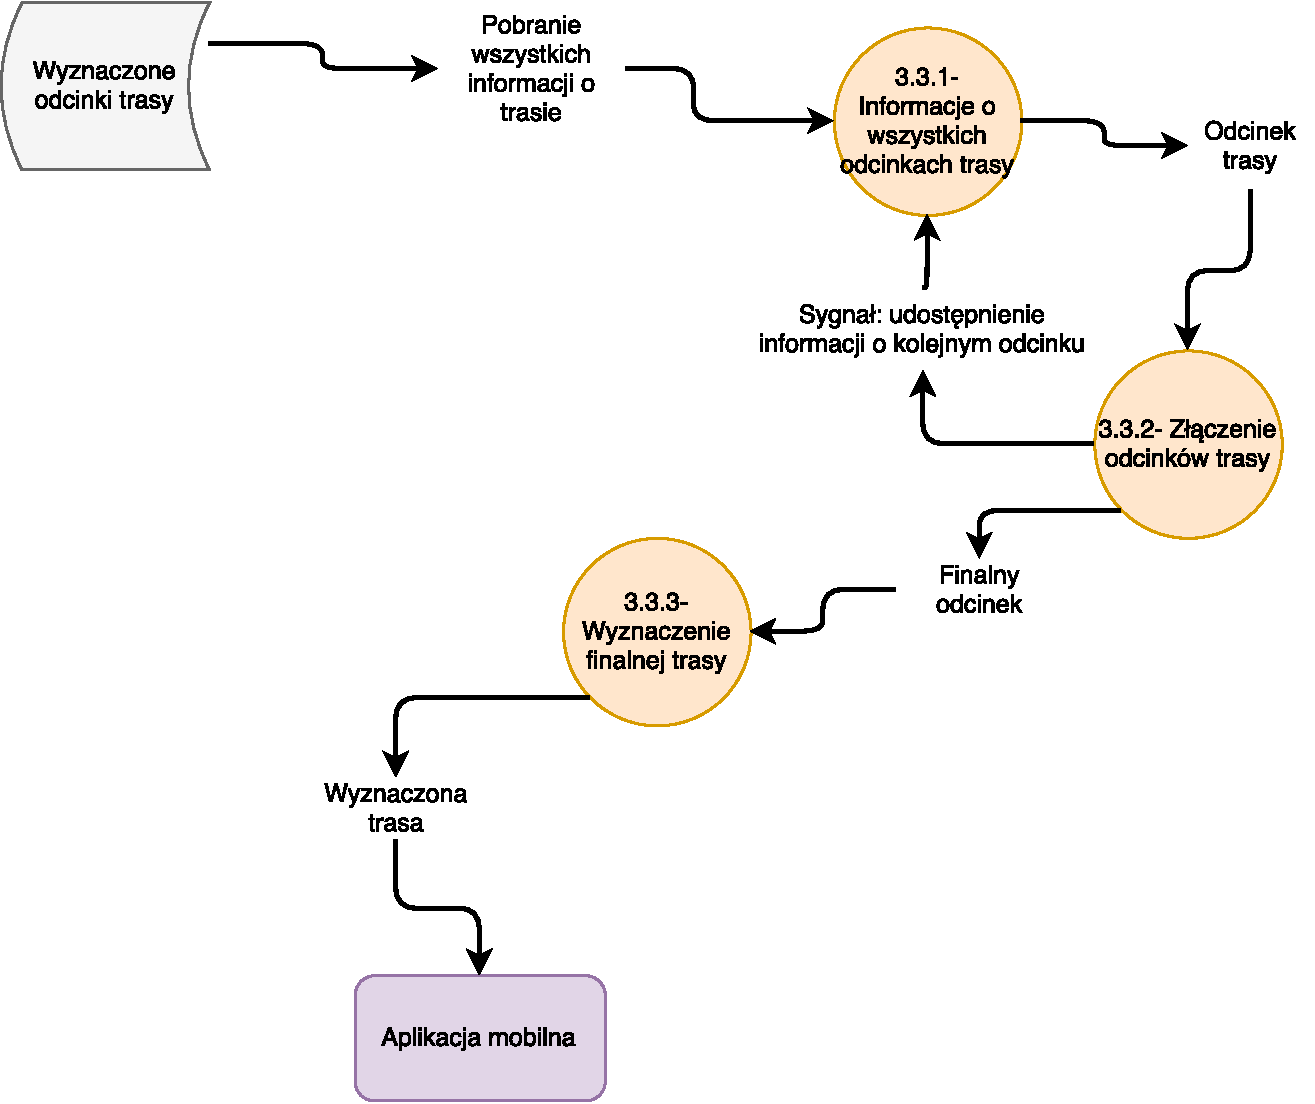
\includegraphics[scale=0.6]{DFD33.pdf}
	\end{center}
	\newpage
	\subsection{DFD 4.1 Obliczanie zmiany położenia}
	\begin{center}
		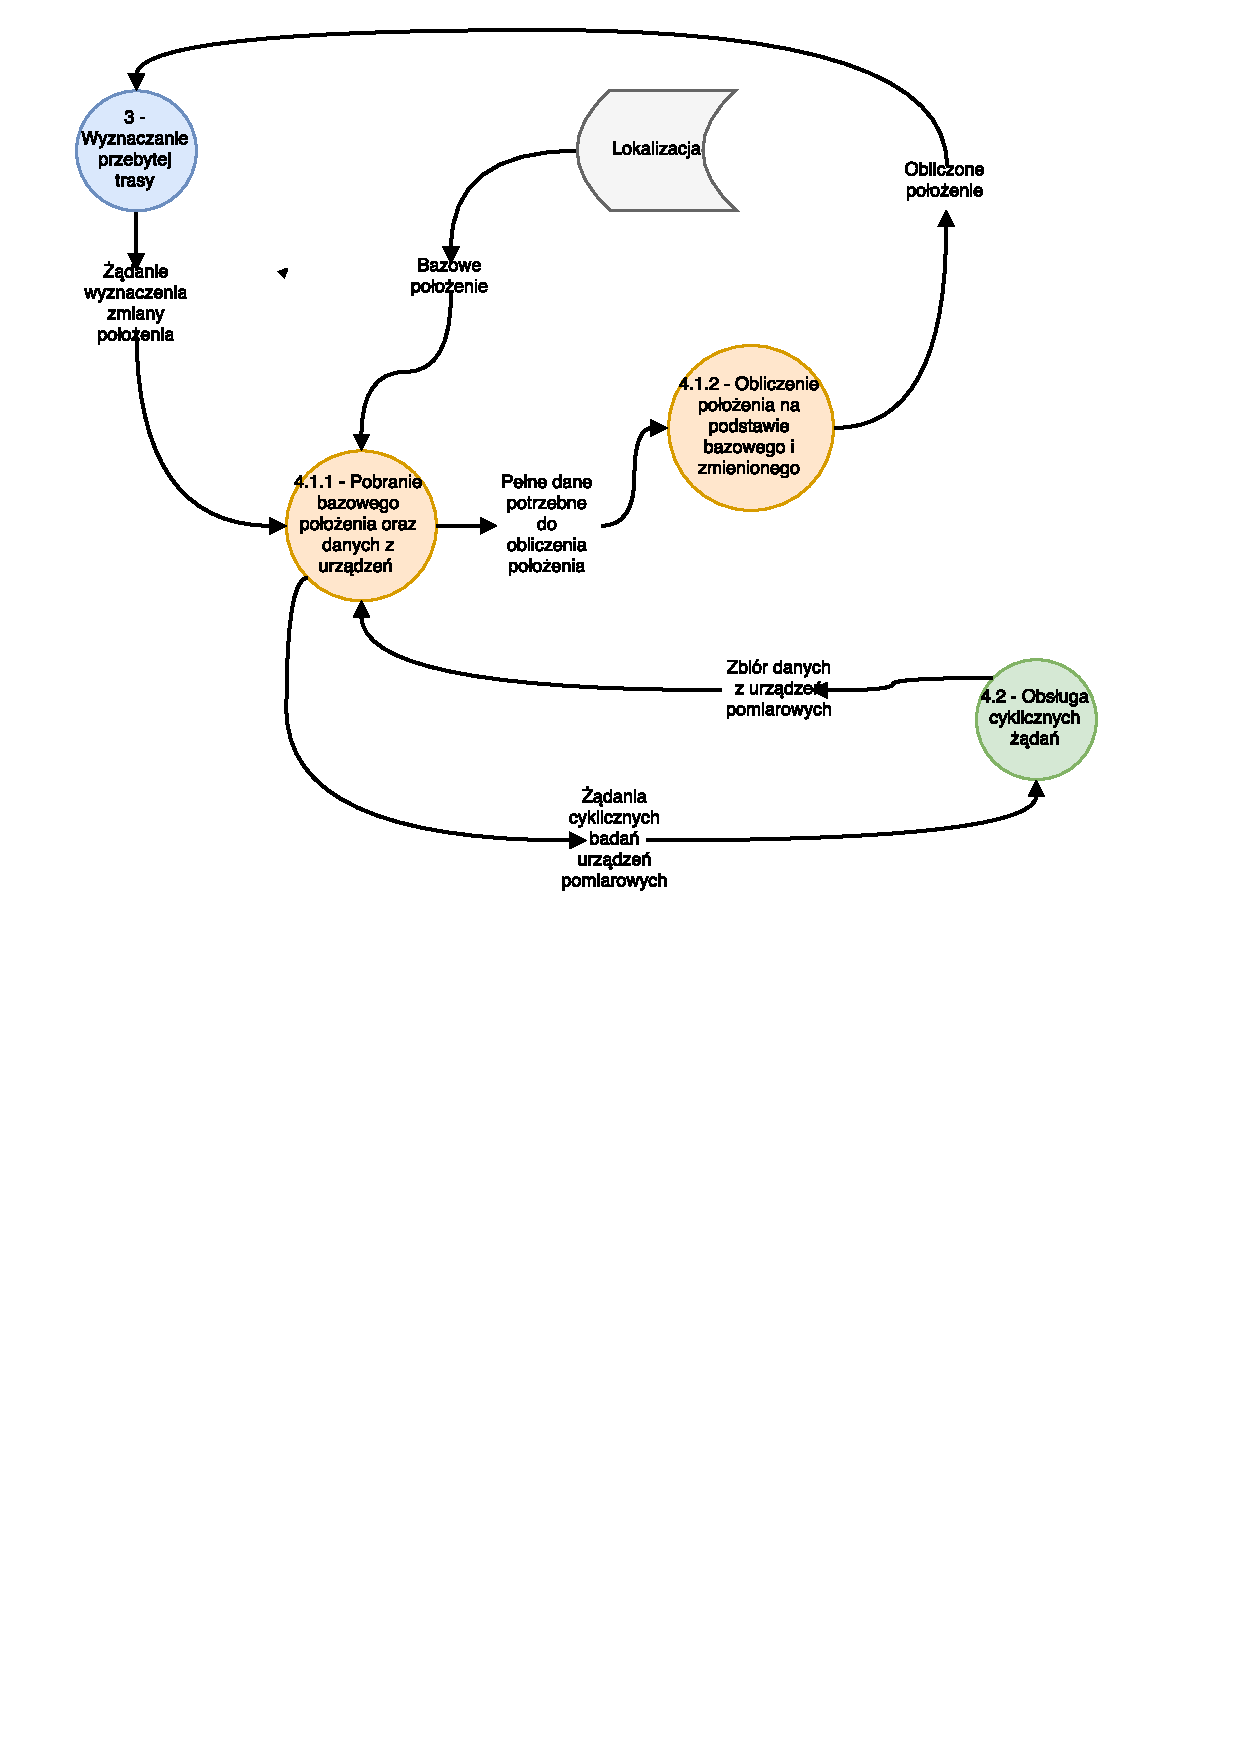
\includegraphics[scale=0.6]{DFD41.pdf}
	\end{center}
	\subsection{DFD 4.2 Obsługa cyklicznych żądań}
	\begin{center}
		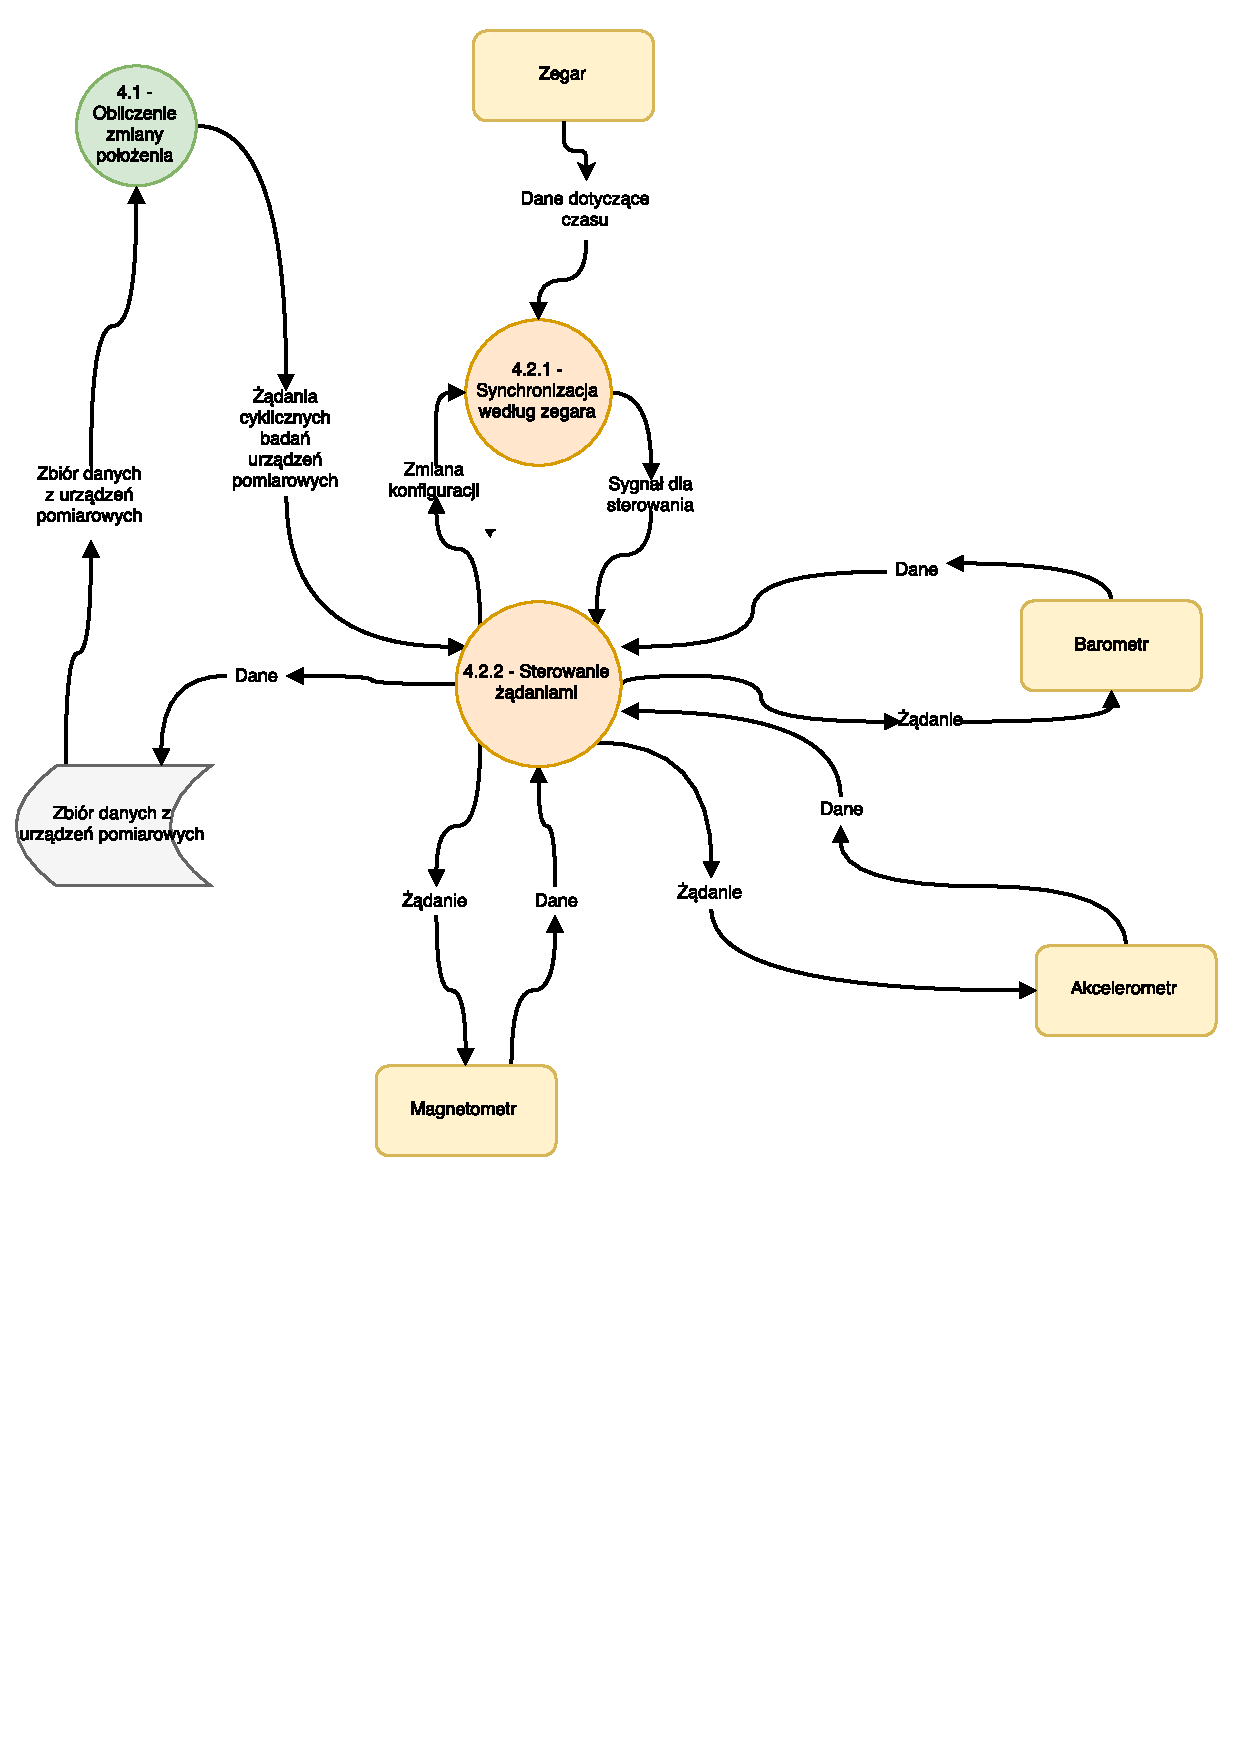
\includegraphics[scale=0.55]{DFD42.pdf}
	\end{center}
	\newpage
	\section{ERD - diagram}
	\begin{center}
		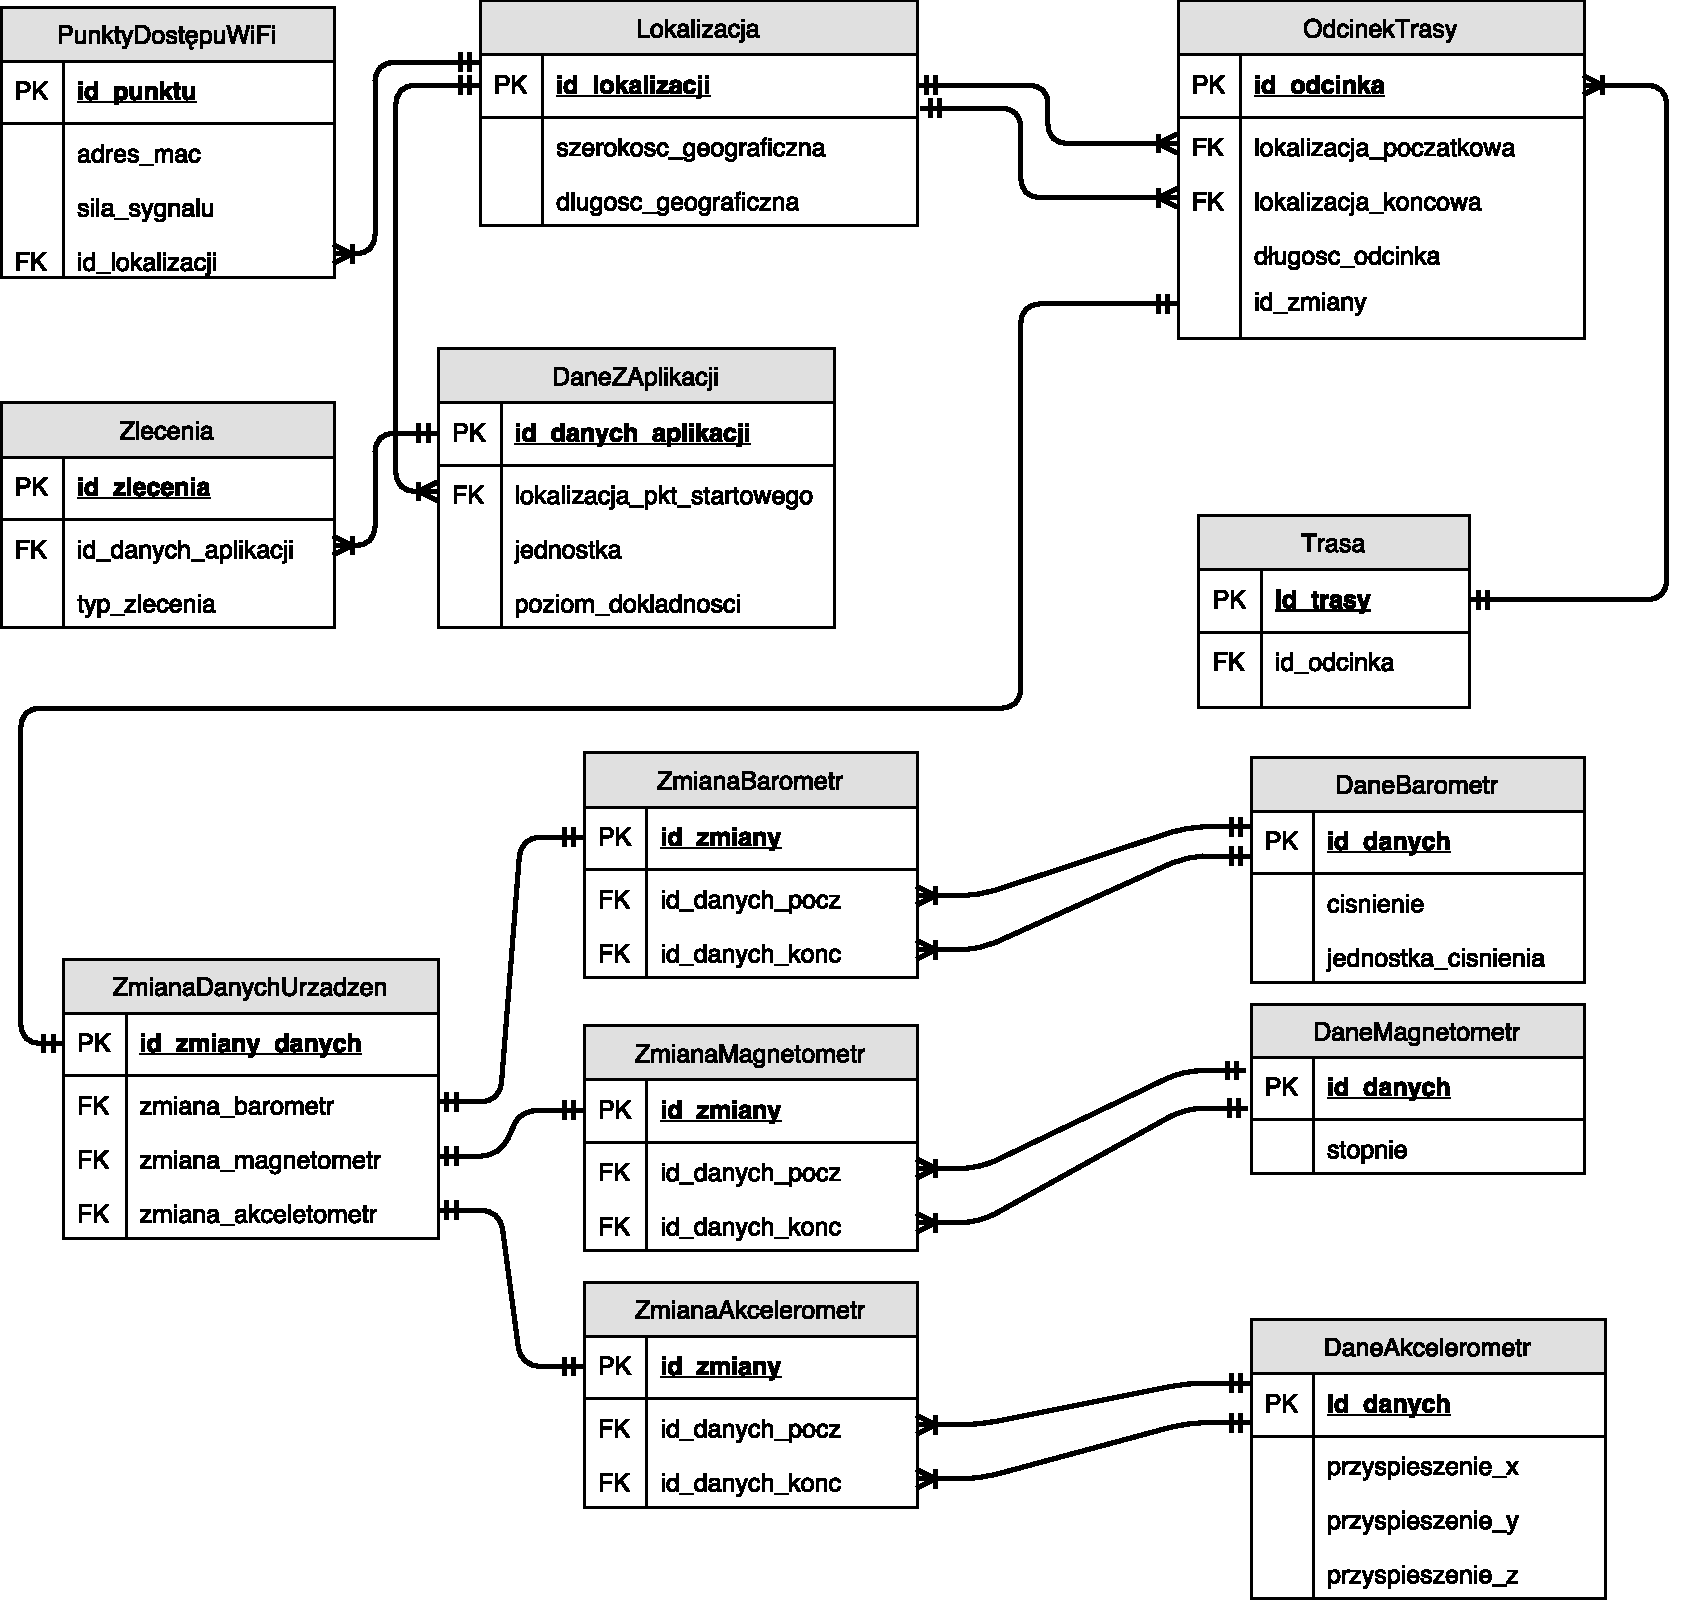
\includegraphics[scale=0.65]{ERD.pdf}
	\end{center}
	\newpage
	\section{ERD - opis}
	\subsection{PunktyDostępuWiFi}
	\begin{center}
		\includegraphics[scale=1]{punktyDostepu.PNG}
	\end{center}
	\subsection{Lokalizacja}
	\begin{center}
		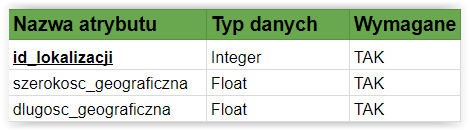
\includegraphics[scale=1]{Lokalizacja.PNG}
	\end{center}
	\subsection{Odcinek}
	\begin{center}
		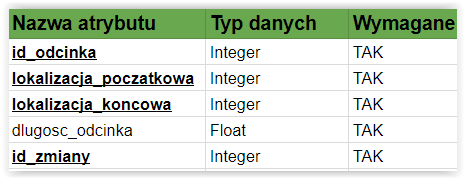
\includegraphics[scale=1]{Odcinek.PNG}
	\end{center}
	\subsection{Trasa}
	\begin{center}
		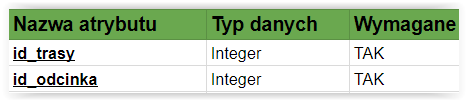
\includegraphics[scale=1]{Trasa.PNG}
	\end{center}
	\subsection{Dane z aplikacji}
	\begin{center}
		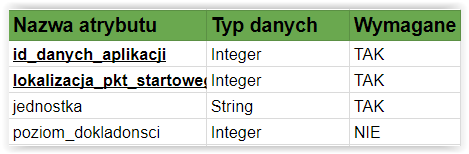
\includegraphics[scale=1]{daneAplikacji.PNG}
	\end{center}
	\subsection{Zlecenia}
	\begin{center}
		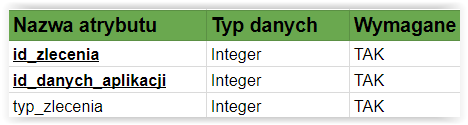
\includegraphics[scale=1]{zlecenia.PNG}
	\end{center}
	\subsection{Dane akcelerometr}
	\begin{center}
		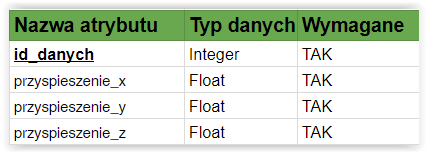
\includegraphics[scale=1]{daneAkcelerometr.PNG}
	\end{center}
	\subsection{Dane magnetometr}
	\begin{center}
		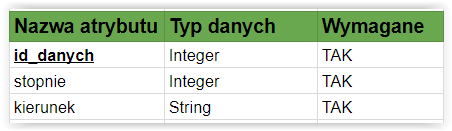
\includegraphics[scale=1]{daneMagnetometr.PNG}
	\end{center}
	\subsection{Dane barometr}
	\begin{center}
		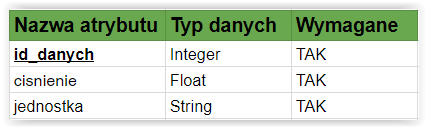
\includegraphics[scale=1]{daneBarometr.PNG}
	\end{center}
	\subsection{Dane zmiana}
	\begin{center}
		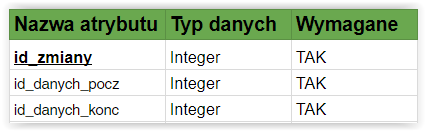
\includegraphics[scale=1]{zmianaBarometr.PNG}
	\end{center}
	\subsection{Zmiana}
	\begin{center}
		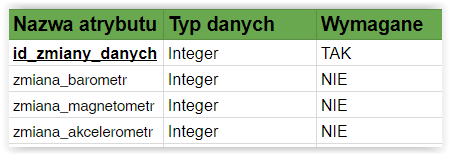
\includegraphics[scale=1]{zmianaDanych.PNG}
	\end{center}
	\newpage
	\section{STD}
	\subsection{STD poziom 0}
	\begin{center}
		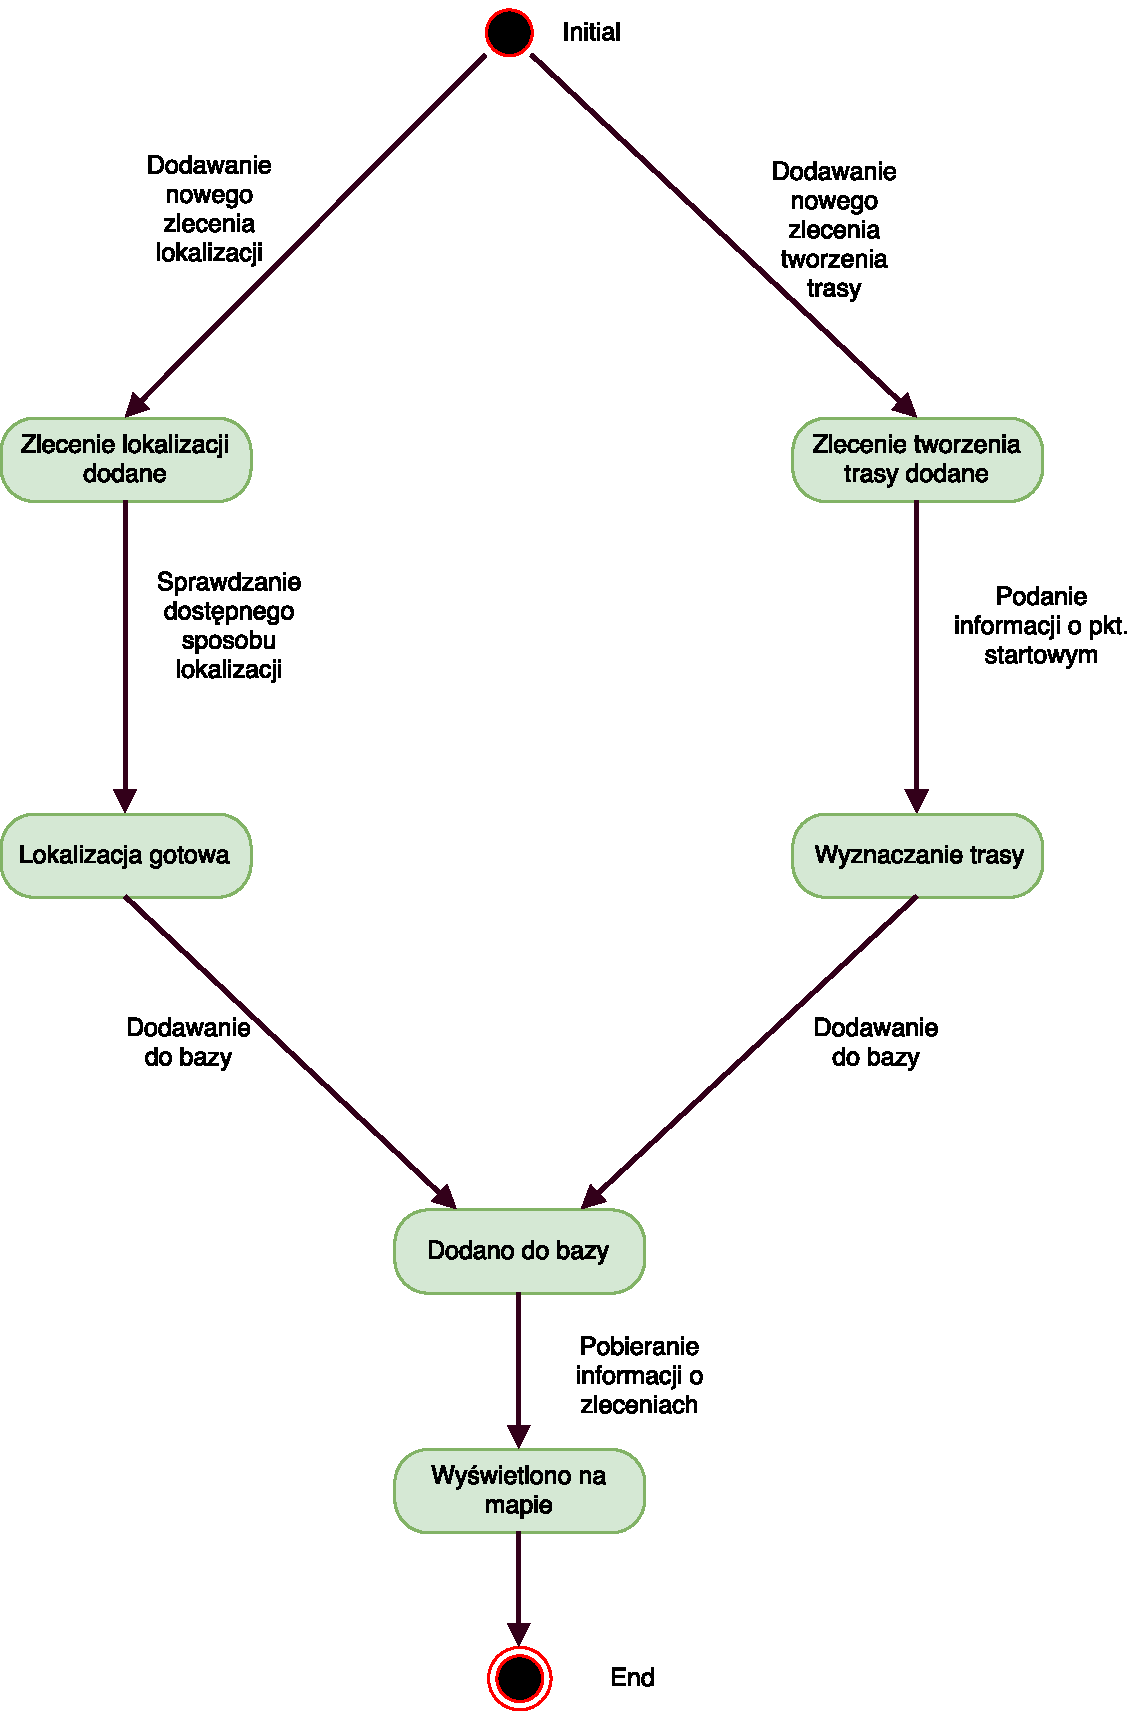
\includegraphics[scale=0.9]{STD0.pdf}
	\end{center}
	\newpage
	\subsection{STD poziom 1 - Lokalizacja gotowa}
	\begin{center}
		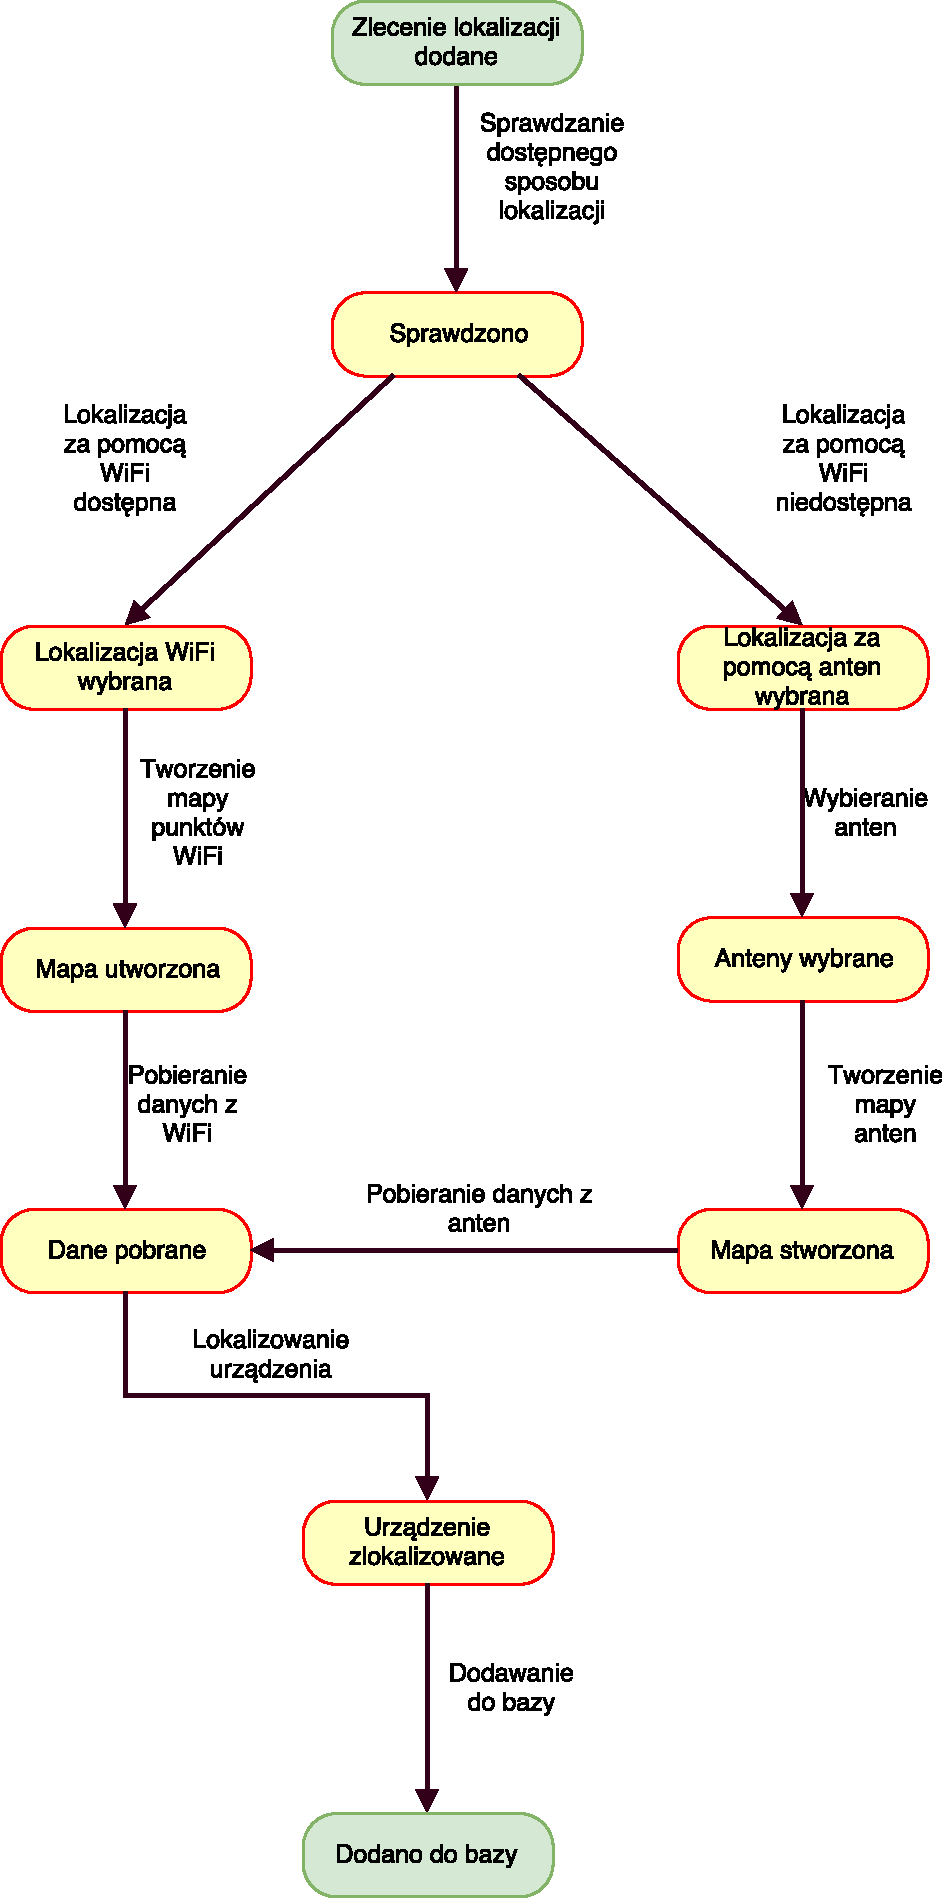
\includegraphics[scale=0.9]{STD1.pdf}
	\end{center}
	\newpage
	\subsection{STD poziom 1 - Trasa gotowa}
	\begin{center}
		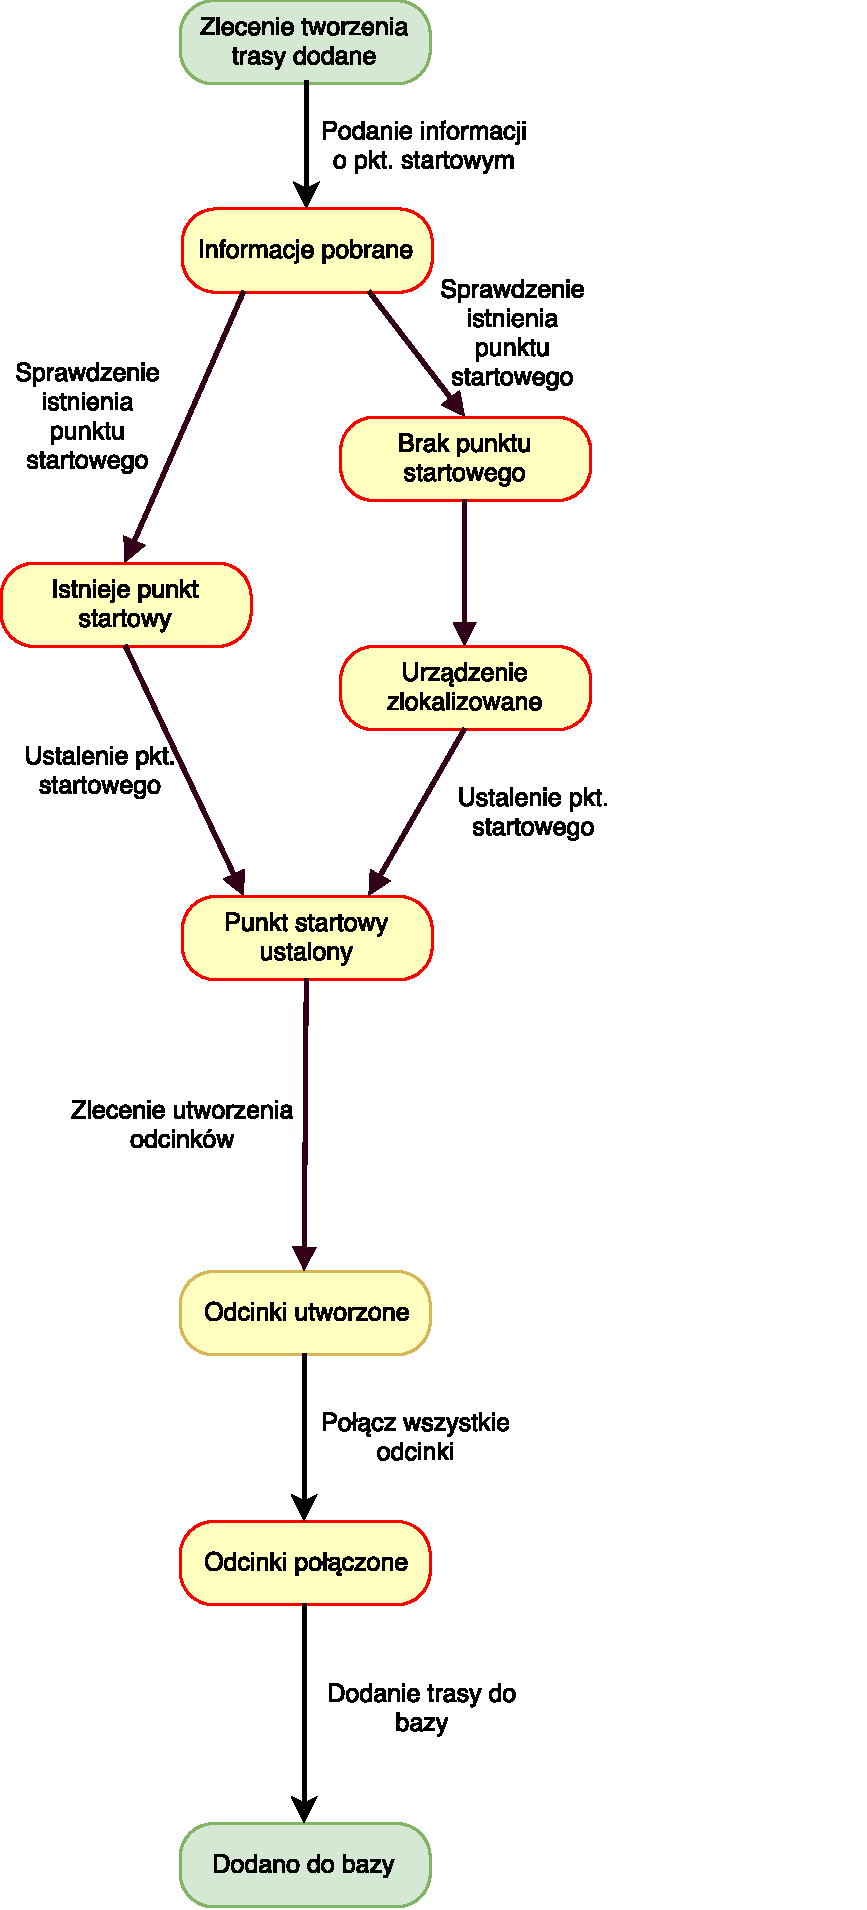
\includegraphics[scale=0.9]{STD2.pdf}
	\end{center}
	\newpage
	\subsection{STD poziom 1 - Wyświetlono na mapie}
	\begin{center}
		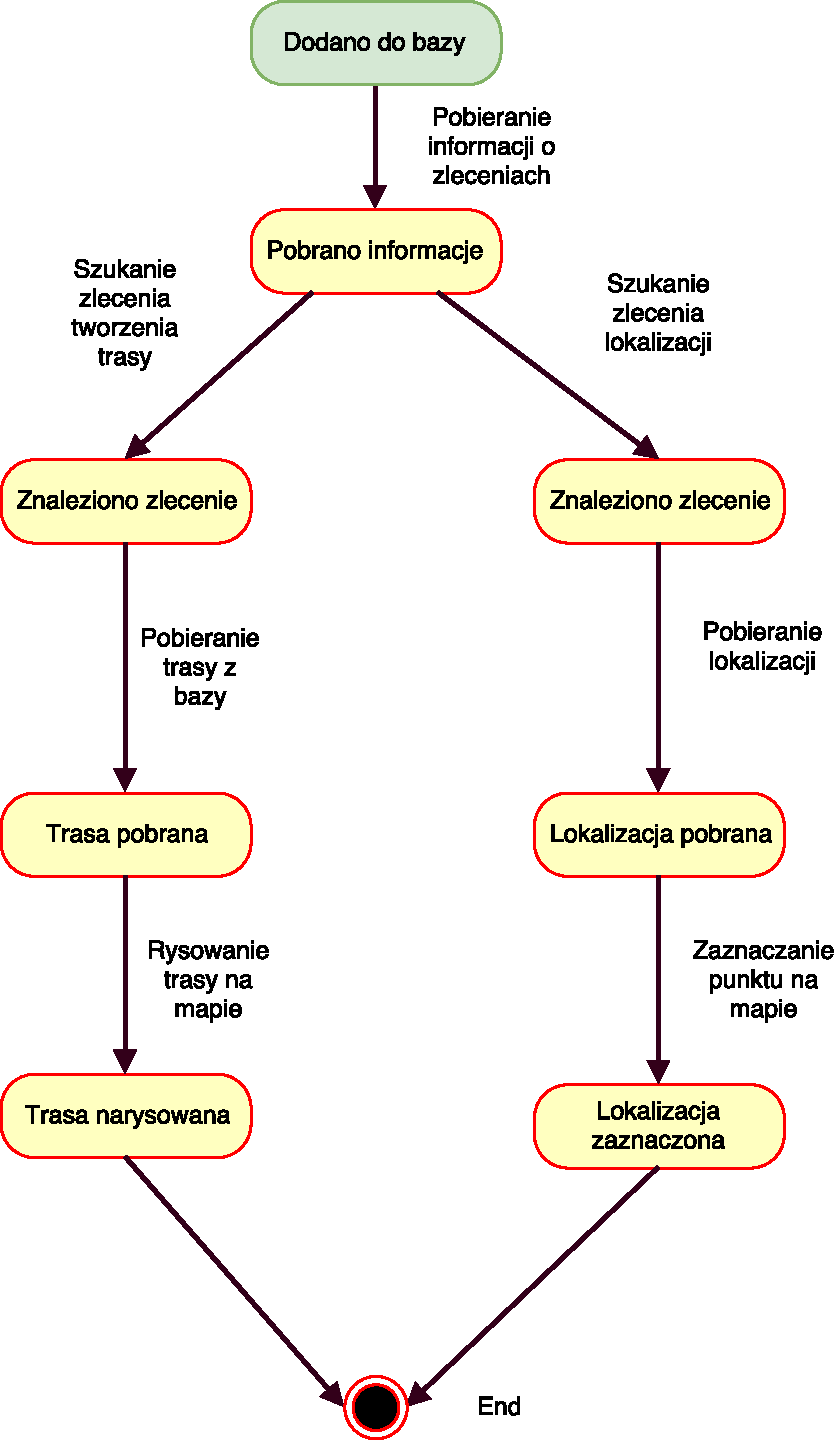
\includegraphics[scale=0.95]{STD3.pdf}
	\end{center}
	\newpage
	\subsection{STD poziom 2 - Odcinki utworzone}
	\begin{center}
		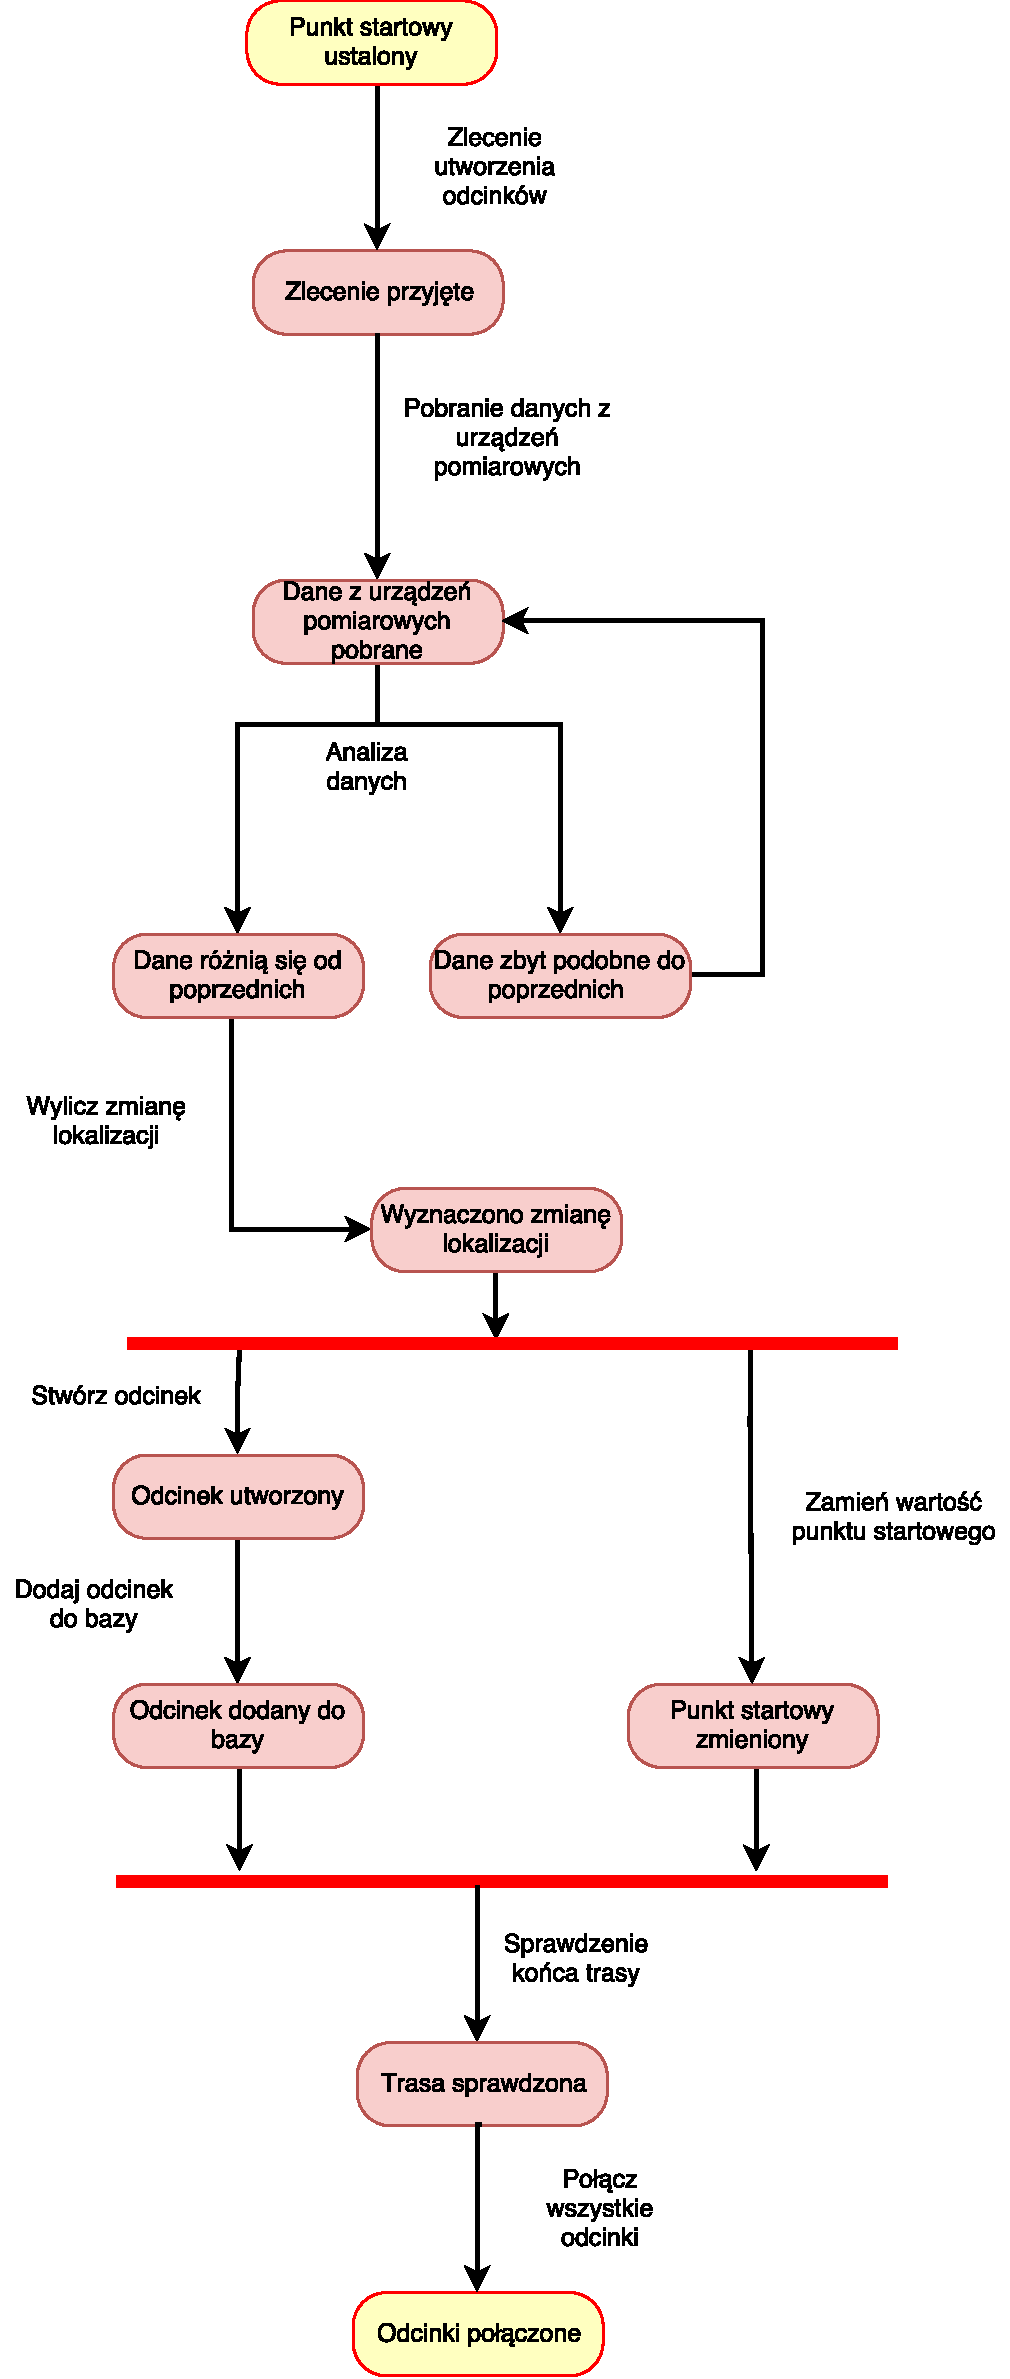
\includegraphics[scale=0.75]{STD4.pdf}
	\end{center}
	\newpage
	\section{Specyfikacja procesów (PSPEC).}
	\begin{enumerate}
		\item Obsługa zleceń.
		\begin{enumerate}[label*=\arabic*.]
			\item Zlecenie wyznaczenia przebytej trasy.
			\begin{enumerate}[label*=\arabic*.]
				\item Wstępna konfiguracja. \newline
				\textbf{Dane wejściowe}: Typ zlecenia od użytkownika, dokładność lokalizacji z danych aplikacji	\newline
				\textbf{Warunek wejściowy}: Typ zlecenia = Zlecenie wyznaczenia trasy		\newline   	
				\textbf{Opis działania}: Przygotowanie konfiguracji do tworzenia trasy. Zapytanie o punkt startowy do bazy oraz wysłanie żądania o przygotowanie zlecenia wyzanaczenia trasy o zadanej dokładności.	\newline
				\textbf{Dane wyjściowe}: Dane na temat konfiguracji.	\newline
				\textbf{Warunek wyjściowy}: Brak
				\item Ustawienia punktu startowego. \newline
				\textbf{Dane wejściowe}: Dane na temat punktu startowego	\newline
				\textbf{Warunek wejściowy}: Brak		\newline   	
				\textbf{Opis działania}: Sprawdzenie czy istnieje już wyznaczony punkt startowy i przekazanie informacji o nim do konfiguracji.	\newline
				\textbf{Dane wyjściowe}: Informacje na temat punktu startowego.	\newline
				\textbf{Warunek wyjściowy}: Brak
				\item Przygotowanie zlecenia wyznaczenia trasy. \newline
				\textbf{Dane wejściowe}: Konfiguracja.	\newline
				\textbf{Warunek wejściowy}: Brak.		\newline   	
				\textbf{Opis działania}: Stworzenie nowego zlecenia w bazie zleceń oraz wysłanie żądania o rozpoczęcie wyzanaczania trasy.	\newline
				\textbf{Dane wyjściowe}: Dane o zleceniu przesyłane do bazy zleceń.	\newline
				\textbf{Warunek wyjściowy}: Brak
			\end{enumerate}
			\item Zlecenie rozpoczęcia lokalizacji urządzenia.
			\begin{enumerate}[label*=\arabic*.]
				\item Wstępna konfiguracja. \newline
				\textbf{Dane wejściowe}: Typ zlecenia od użytkownika, dokładność lokalizacji z danych aplikacji	\newline
				\textbf{Warunek wejściowy}: Typ zlecenia = Zlecenie lokalizacji		\newline   	
				\textbf{Opis działania}: Przygotowanie konfiguracji do lokalizacji urządzenia o zadanej dokładności.	\newline
				\textbf{Dane wyjściowe}: Konfiguracja.	\newline
				\textbf{Warunek wyjściowy}: Brak.
				\item Przygotowanie zlecenia wyznaczenia lokalizacji. \newline
				\textbf{Dane wejściowe}: Konfiguracja.	\newline
				\textbf{Warunek wejściowy}: Brak		\newline   	
				\textbf{Opis działania}: Tworzenie nowego zlecenia o lokalizcji i umieszczenie go w bazie zleceń oraz wysłanie żądania o rozpoczęcie lokalizowania.	\newline
				\textbf{Dane wyjściowe}: Dane o zleceniu przesyłane do bazy zleceń.	\newline
				\textbf{Warunek wyjściowy}: Brak
			\end{enumerate}
		\end{enumerate}
		\item Lokalizowanie.
		\begin{enumerate}[label*=\arabic*.]
			\item Sprawdzanie dostępnego sposobu lokalizacji.
			\begin{enumerate}[label*=\arabic*.]
				\item Sprawdzanie dostępności punktów WiFi. \newline
				\textbf{Dane wejściowe}: Typ zlecenia	\newline
				\textbf{Warunek wejściowy}: Typ zlecenia = Zlecenie lokalizacji		\newline   	
				\textbf{Opis działania}: Szukanie dostępnych punktów WiFi, sprawdzanie mocy ich sygnału. 	\newline
				\textbf{Dane wyjściowe}: Dane na temat dostępności.	\newline
				\textbf{Warunek wyjściowy}: Brak
				\item Sprawdzanie dostępności masztów telefonii komórkowej. \newline
				\textbf{Dane wejściowe}: 	\newline
				\textbf{Warunek wejściowy}: Brak		\newline   	
				\textbf{Opis działania}: Szukanie dostępnych masztów telefonii komórkowej, porównywanie ich syganału.	\newline
				\textbf{Dane wyjściowe}: Dane na temat dostępności.	\newline
				\textbf{Warunek wyjściowy}: Brak
				\item Wybranie dostępnego sposobu. \newline
				\textbf{Dane wejściowe}: Dane na temat dostępności punktów Wifi i masztów telefonii komórkowej	\newline
				\textbf{Warunek wejściowy}: Brak		\newline   	
				\textbf{Opis działania}: Wybranie najlepszego dostępnego sposobu lokalizacji.	\newline
				\textbf{Dane wyjściowe}: Dane na temat lepszego sposobu.	\newline
				\textbf{Warunek wyjściowy}: Brak
			\end{enumerate}
			\item Lokalizacja za pomocą WiFi.
			\begin{enumerate}[label*=\arabic*.]
				\item Stworzenie mapy punktów WiFi. \newline
				\textbf{Dane wejściowe}: Dane o punktach WiFi z bazy danych.	\newline
				\textbf{Warunek wejściowy}: Brak	\newline   	
				\textbf{Opis działania}: Tworzenie mapy punktów WiFi na podstawie informacji o ich położeniu z bazy danych.	\newline
				\textbf{Dane wyjściowe}: Mapa punktów WiFi.	\newline
				\textbf{Warunek wyjściowy}: Brak
				\item Wyliczanie położenia. \newline
				\textbf{Dane wejściowe}: Mapa punktów WiFi, Dane z WiFi	\newline
				\textbf{Warunek wejściowy}: Brak		\newline   	
				\textbf{Opis działania}: Na podstawie otrzymanej mapy punktów WiFi oraz danych pobieranych z tych punktów wyznaczana jest lokalizacja o wyliczonym przybliżeniu.	\newline
				\textbf{Dane wyjściowe}: Lokalizacja	\newline
				\textbf{Warunek wyjściowy}: Brak
			\end{enumerate}
			\item Lokalizacja za pomocą masztów telefonii komórkowej.
			\begin{enumerate}[label*=\arabic*.]
				\item Wybranie masztów o najlepszej mocy sygnału. \newline
				\textbf{Dane wejściowe}: Dostępne maszty	\newline
				\textbf{Warunek wejściowy}:  Brak		\newline   	
				\textbf{Opis działania}: Porównywanie dostępnych masztów i wybranie tych o najsilniejszym sygnale oraz stworzenie z nich mapy.	\newline
				\textbf{Dane wyjściowe}: Mapa masztów telefonii komórkowej.  	\newline
				\textbf{Warunek wyjściowy}:Brak
				\item Wyliczanie położenia. \newline
				\textbf{Dane wejściowe}: Mapa masztów telefonii komórkowej , Dane z masztów	\newline
				\textbf{Warunek wejściowy}: Brak		\newline   	
				\textbf{Opis działania}: Na podstawie otrzymanej mapy oraz danych pobieranych z masztów telefonii komórkowej wyznaczana jest lokalizacja o wyliczonym przybliżeniu.	\newline
				\textbf{Dane wyjściowe}: Lokalizacja	\newline
				\textbf{Warunek wyjściowy}: Brak
			\end{enumerate}
		\end{enumerate}
		\item Wyznacznie przebytej trasy.
		\begin{enumerate}[label*=\arabic*.]
			\item Obsługa cyklicznych zmian położenia.
			\begin{enumerate}[label*=\arabic*.]
		   	\item Sterowanie zmianami. \newline
				\textbf{Dane wejściowe}:	\newline
				\textbf{Warunek wejściowy}: 		\newline   	
				\textbf{Opis działania}:	\newline
				\textbf{Dane wyjściowe}:	\newline
				\textbf{Warunek wyjściowy}:
				\item Konfiguracja. \newline
				\textbf{Dane wejściowe}:	\newline
				\textbf{Warunek wejściowy}: 		\newline   	
				\textbf{Opis działania}:	\newline
				\textbf{Dane wyjściowe}:	\newline
				\textbf{Warunek wyjściowy}:
				\item Synchronizacja według zegara. \newline
				\textbf{Dane wejściowe}:	\newline
				\textbf{Warunek wejściowy}: 		\newline   	
				\textbf{Opis działania}:	\newline
				\textbf{Dane wyjściowe}:	\newline
				\textbf{Warunek wyjściowy}:
			\end{enumerate}
			\item Wyliczanie poszczególnej przebytej trasy.
			\begin{enumerate}[label*=\arabic*.]
				\item Ustalenia położenia według urządzenia lokalizującego. \newline
				\textbf{Dane wejściowe}:	\newline
				\textbf{Warunek wejściowy}: 		\newline   	
				\textbf{Opis działania}:	\newline
				\textbf{Dane wyjściowe}:	\newline
				\textbf{Warunek wyjściowy}:
				\item Ustalenie położenia według urządzeń pomiarowych. \newline
				\textbf{Dane wejściowe}:	\newline
				\textbf{Warunek wejściowy}: 		\newline   	
				\textbf{Opis działania}:	\newline
				\textbf{Dane wyjściowe}:	\newline
				\textbf{Warunek wyjściowy}:
				\item Wyliczenie błędu pomiarowego. \newline
				\textbf{Dane wejściowe}:	\newline
				\textbf{Warunek wejściowy}: 		\newline   	
				\textbf{Opis działania}:	\newline
				\textbf{Dane wyjściowe}:	\newline
				\textbf{Warunek wyjściowy}:
				\item Wyznaczenie trasy. \newline
				\textbf{Dane wejściowe}:	\newline
				\textbf{Warunek wejściowy}: 		\newline   	
				\textbf{Opis działania}:	\newline
				\textbf{Dane wyjściowe}:	\newline
				\textbf{Warunek wyjściowy}:
			\end{enumerate}
			\item Wyznaczanie całej przebytej trasy.
			\begin{enumerate}[label*=\arabic*.]
				\item Informacje o wszystkich odcinkach trasy. \newline
				\textbf{Dane wejściowe}:	\newline
				\textbf{Warunek wejściowy}: 		\newline   	
				\textbf{Opis działania}:	\newline
				\textbf{Dane wyjściowe}:	\newline
				\textbf{Warunek wyjściowy}:
				\item Złączenie odcinków trasy. \newline
				\textbf{Dane wejściowe}:	\newline
				\textbf{Warunek wejściowy}: 		\newline   	
				\textbf{Opis działania}:	\newline
				\textbf{Dane wyjściowe}:	\newline
				\textbf{Warunek wyjściowy}:
				\item Wyzanczenie finalnej trasy. \newline
				\textbf{Dane wejściowe}:	\newline
				\textbf{Warunek wejściowy}: 		\newline   	
				\textbf{Opis działania}:	\newline
				\textbf{Dane wyjściowe}:	\newline
				\textbf{Warunek wyjściowy}:
			\end{enumerate}
		\end{enumerate}
		\item Obsługa zmiany położenia.
		\begin{enumerate}[label*=\arabic*.]
			\item Obliczanie zmiany położenia.
			\begin{enumerate}[label*=\arabic*.]
				\item Pobranie bazowego położenia oraz danych z urządzeń. \newline
				\textbf{Dane wejściowe}: Bazowe położenie pobrane z bazy, zbiór danych z urządzeń pomiarowych	\newline
				\textbf{Warunek wejściowy}: Brak		\newline   	
				\textbf{Opis działania}: Pobranie bazowego położenia z bazy oraz żądanie o cykliczne dane z urządzeń pomiaowych. Stworzenie na ich podstawie danych do obliczenia zmiany położenia.	\newline
				\textbf{Dane wyjściowe}: Dane potrzebne do obliczenia zmiany położenia.	\newline
				\textbf{Warunek wyjściowy}: Brak
				\item Obliczanie położenia na podstawie bazowego i zmienionego. \newline
				\textbf{Dane wejściowe}:Dane potrzebne do obliczenia zmiany położenia.	\newline
				\textbf{Warunek wejściowy}: Brak		\newline   	
				\textbf{Opis działania}: Obliczenie położenia na podstawie otrzymanych danych. Bazowe położenie + zmiana położenie.	\newline
				\textbf{Dane wyjściowe}: Nowe położenie.	\newline
				\textbf{Warunek wyjściowy}: Brak
			\end{enumerate}
			\item Obsługa cyklicznych żądań.
			\begin{enumerate}[label*=\arabic*.]
				\item Synchronizacja według zegara. \newline
				\textbf{Dane wejściowe}: Dane na temat czasu od zegara.	\newline
				\textbf{Warunek wejściowy}:  Brak		\newline   	
				\textbf{Opis działania}: Generowanie sygnału dla sterowania o zadanaej częstotliwości.	\newline
				\textbf{Dane wyjściowe}: Cykliczne cygnały.	\newline
				\textbf{Warunek wyjściowy}: Brak
				\item Sterowanie żądaniami. \newline
				\textbf{Dane wejściowe}: Cykliczne sygnały.	\newline
				\textbf{Warunek wejściowy}: Brak.		\newline   	
				\textbf{Opis działania}: Po otrzymaniu nowego sygnału wysyłanie zapytań do urządzeń pomiarowych o dane.	\newline
				\textbf{Dane wyjściowe}: Dane z urządzeń pomiarowych.	\newline
				\textbf{Warunek wyjściowy}: Brak
			\end{enumerate}
		\end{enumerate}
	\end{enumerate}
\end{document}